% Chapter 7

\chapter{Social and spatial inequalities in commuter energy use} % Write in 
\label{Chapter7}
% \lhead{Chapter 7. \emph{Social and spatial inequalities in commuter energy
% use}}
\fancyhead[RO,LE]{Chapter 7. Social and spatial inequalities} %2side
\fancyhead[RE,LO]{\thepage}
% Latest plan (May) --- add complete vulnerability paper in here to save time
\begin{quotation}
\textit{ There  are many options open  for manipulation of the transportation
system,
and many  impacts on different groups which must
be considered. Prediction of the impacts associated with
a particular set of options requires prediction of the corresponding
pattern of flows which will occur in the multimodal transportation
network, using a complex system of models.}
\end{quotation} {\flushright \citep{manheim1968search}}

\section{The importance of distributional impacts in transport studies}
At the sub-national level, the relative costs and benefits of climate change-related
policies are highly uneven. It has been calculated, for example that the bottom
10\% of households by income will benefit least from the government's domestic
energy policies such as those contained in the Green Deal \citep{JRF2013-distributions}.
This, the authors point out, is unfair on three levels: poor people are least
able to deal with the impacts of climate change; they pay proportionally more for the
mitigation strategies; yet they have contributed least to the problem: the top
10\% emit 3 times more emissions than the bottom 10\%, excluding indirect emissions
caused by the products and services they consume.

At the aggregate level, literature shows that behaviour varies depending
on a range of factors including distance to employment
centres,
transport infrastructure and the number of local employment opportunities.
Social characteristics are also closely linked with commuting behaviour,
as illustrated by DfT data on the average distance travelled to work
by mode, cross tabulated by household income (\cref{fig:income-dis}). Transport
modelling, and especially the related discipline of transport engineering, have
tended to be `hard' subjects, focussed only on the technological performance of
transport interventions. However, as implied by the quote that begins this
chapter, \emph{all} transport interventions will have some kind of
distributional impacts, either favouring certain places more than others or
certain groups of people.

The dangers of omitting such social considerations from the analysis were
recognised early in the history of transport and urban modelling. In fact,
ignorance of distributional impacts was implicated as
one of the reasons for the perceived failure of the first generation of urban
models in the 1960s: ``disillusionment with technology began to grow as
planners and politicians began to realise that long-term planning of
transportation and land use [which the models focussed on] had little or nothing
to do with more immediate problems of poverty and inequality''
\citep[p~10]{batty1976urban}. This problem continues today (see
\citealp{Tribby2012} for one example), providing a strong remit for this
chapter and its focus on including social factors in the evaluation of travel
patterns and future interventions. Before moving on to the core results of this
chapter --- a case study of inequalities in commuting patterns and energy used
in South Yorkshire --- it is worth considering a few national statistics on
the relationship between socio-economic variables and transport to work, for
context.

\begin{figure}[htbp]
  \centerline{
    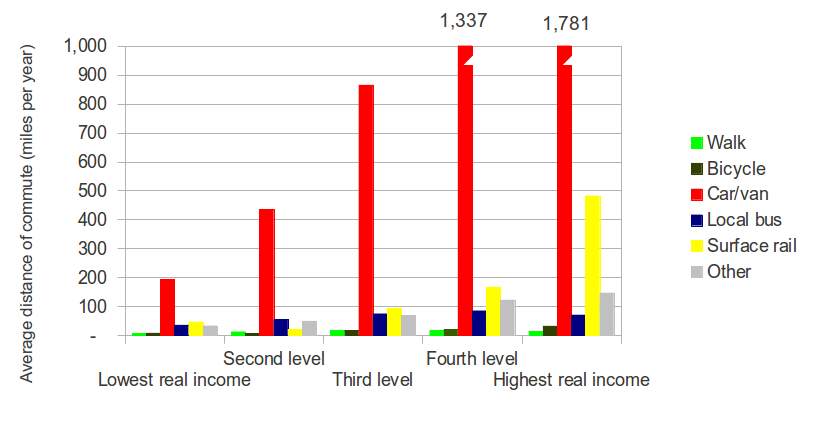
\includegraphics[width = 14 cm]{./Figures/Income-dis-GB}}
    \rule{35em}{0.5pt}
  \caption[Trip distance and mode by household income]{Average
distance of commute by mode by income quintiles in Great Britain
in 2009. Data: \citep[Table 6]{DfT2011-commuting}.}
  \label{fig:income-dis}
\end{figure}

\Cref{fig:income-dis} illustrates that social inequalities are manifested
not only in income and material goods but also in terms of the
daily trip to work. Workers in the top 20\% of households by income
commuted on average 8 times further during 2009 than those from the
bottom 20\%. From one income quintile to the next, average distance
almost doubles in every case, with the difference slowing only slightly towards
the
top quintiles.\footnote{Distance
travelled to work increased by a
factor of 1.8, 2.0, 1.5 and 1.4 between Q1 and Q2 in the
first instance to Q4 and Q5 in the last.
}
It is notable from \cref{fig:income-dis} that wealthier people
also tend to use more energy-intensive modes. However,
the variability in mode of transport is far lower than the
variability in distance (\cref{income-heatmap}).

\begin{figure}[htbp]
  \centerline{
    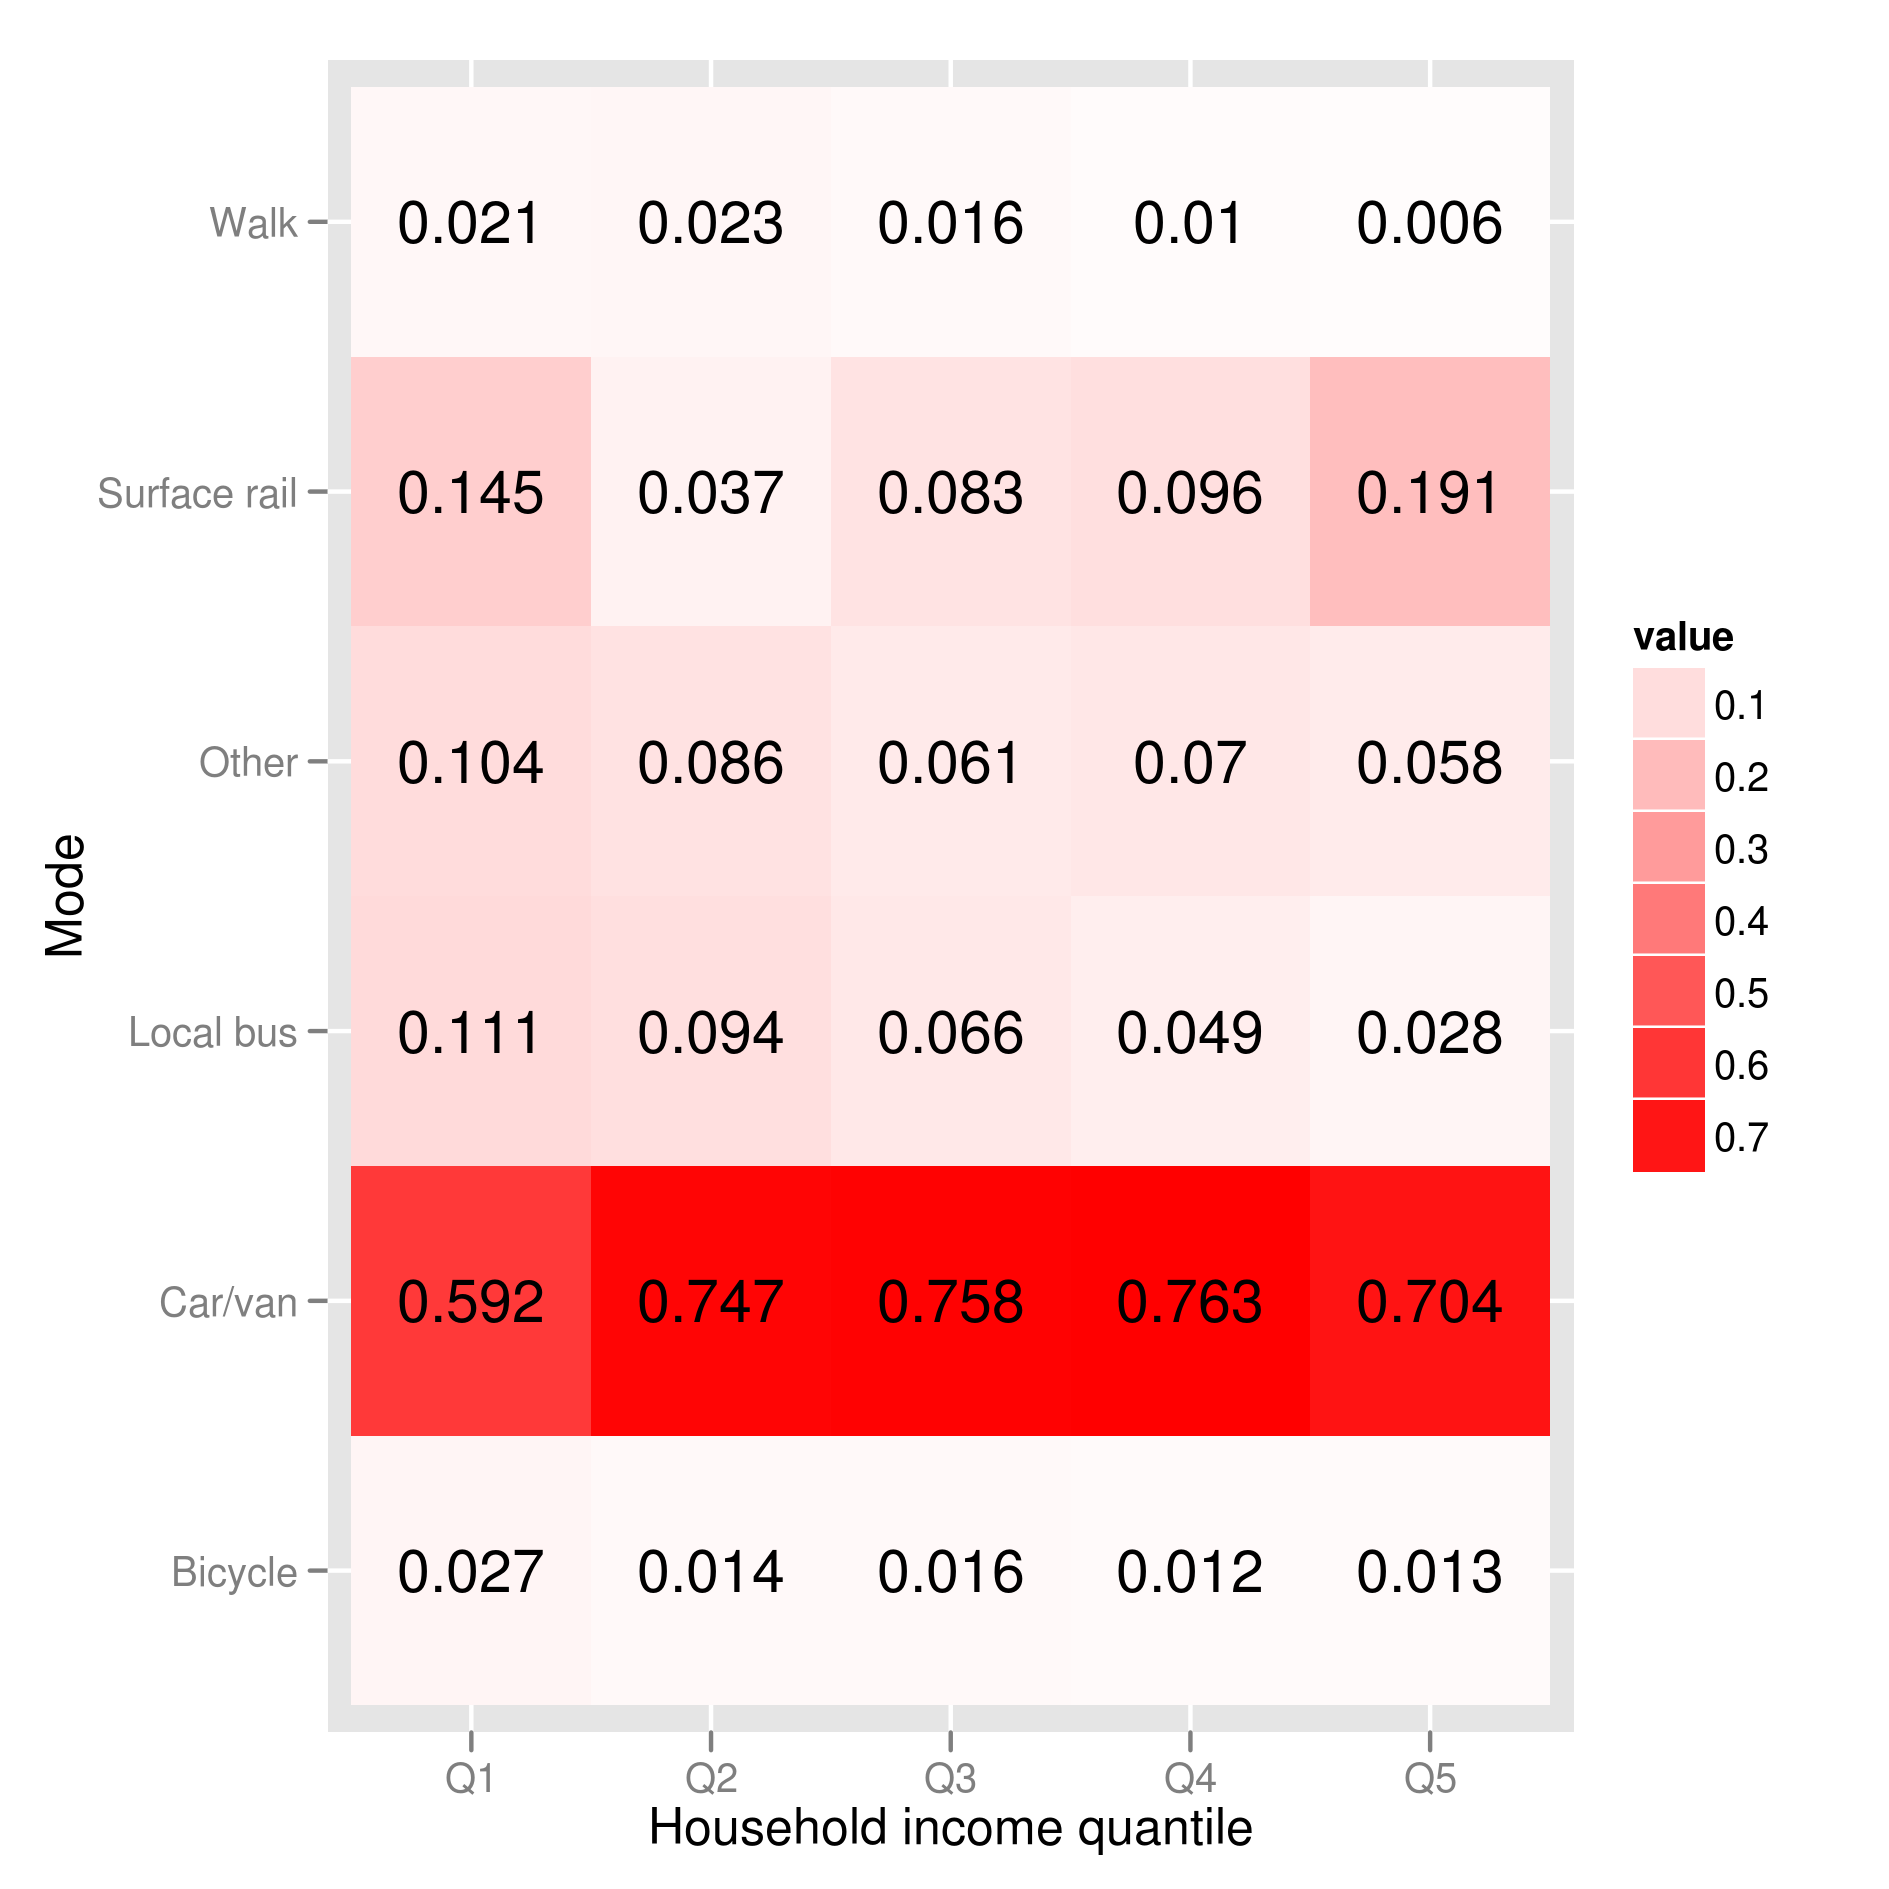
\includegraphics[width = 14 cm]{./Figures/income-heatmap}}
    \rule{35em}{0.5pt}
  \caption[Heatmap of mode of travel by income group]{Proportions
of trips made by mode of transport in Great Britain, 2009.
Data: \citep[Table 6]{DfT2011-commuting}.}
  \label{income-heatmap}
\end{figure}

These overall findings provide a strong message to policy makers:
policies encouraging behavioural change may be most effective
if they target particular groups of commuters.
This differs from blanket policies such as efficiency-related
tax bands which inherently assume commuter patterns are homogeneous.
At sub-national level, such variability depending on socio-economic
status should also be taken into account by local planners.
However, in many cases, the data or analysis capabilities are
not available to target particular groups living in particular areas.

With these motivations, the present chapter builds on the kind of breakdowns in
commuter behaviour
by socio-economic variables illustrated in \cref{fig:income-dis}, but
at lower levels. This is where the simulated individuals provided by
spatial microsimulation really come into their own, as aggregate data tell
us little about the socio-economic attributes of the individuals
that make up aggregate commuter patterns.

The following presents results which tackle these issues.
Because the spatial microsimulation model assigns characteristics to every single
working person in the study area, the analysis becomes unwieldy when applied to
very large areas. (The IPF model took 30 minutes per iteration when applied
to the 2 million commuters of Yorkshire and the Humber on an Intel i5 `Sandy
Bridge' computer with 12 Gb RAM). Age/sex, mode,
distance and social class categories were used as the constraints, from which
a wide range of simulated results were generated.

% \section{A case study of commuting in South Yorkshire}
%%% Try inserting all JTRG paper here - done (ish) how do I reference this???
As noted in chapters 1 and 2, commuting is a major reason for personal travel,
and a broad research area within transport geography. In many cases zonally
aggregated census statistics --- often the most reliable source of
information about spatial variation in commuter patterns --- form the basis of
geographical commuting research
\citep{Horner2002,Titheridge2006}.
Advances in data availability
and computational methods  have facilitated
the analysis at the individual level, as outlined in \cref{Chapter4}.
This trend --- towards micro level social and spatial analysis
--- has several potential benefits
for decision makers. It is the aim of this section to highlight these benefits
and provide useful insights into the link between socio-economic attributes
and commuter behaviour. The case study region of South Yorkshire is the same
as that used in \cref{Chapter6}, for continuity. The results showcase the
potential benefits of spatial microsimulation:
\begin{itemize}
 \item the ability to target specific \emph{types} of commuters
\item the possibility of modelling the impacts of small scale interventions
(e.g.~a new bicycle path or bus lane) on individuals living in the local area
\item higher spatial resolution than is provided by aggregate data for certain
cross-tabulated variables (e.g.~mode and distance). This could provide insight
into the impacts of change on network usage (e.g.~identify likely points of
congestion)
\item a foundation for agent-based and dynamic microsimulation models.
\end{itemize}
% Maybe add refs here.

The shift towards micro level analysis also has some potential
disadvantages. These limitations,
and strategies to overcome them, can be summarised as follows:
\begin{itemize}
 \item The individual level results are simulated, and are unlikely to be
 totally representative of the zones in question. We can have confidence
 in the constrained variables (although large bin sizes for continuous
 attributes such as age may not fully capture unusual
 distributions),\footnote{The
 distance bins presented in Table \ref{t:constraints}, for example,
 are quite widely spaced. In a situation where many people
 travelled a distance close to the edges of one of these bins --- for example
 due to a factory located 11 km from an employment centre --- the results,
 which would represent an even distribution of
 all individuals in the sample who 10 to 20 km to work, would
 be inaccurate.}
 but the target variables are simply the result of their relationship with
 constraint variables at the national level. This can be tackled through
 validation methods (see \citealp{Edwards2009}, and
 below) or, in the long run, through increased access to real spatially
 disaggregated
 microdata.\footnote{For example, a dataset of geo-coded
individuals and their workplaces provided by Finnish government allows
destination/origin analysis and insights into the directions of flow
\citep{Helminen2007}
}
In fact, awareness of the policy insights offered to researchers
by spatial microdata could encourage the release of real
geographically disaggregated microdata (see \citep{Lee2009}).
% \item Better energy data - limitations with EU ways of measuring things,
% discrepancies between DfT data and DECC data.
\item Lack of accurate distance travelled estimates in the main model
(currently broad distance categories are used). This could be overcome by creating
more accurate origin-destination pairs for individuals. Lower level commuter
flow data (compared with the data presented in Fig.~\ref{fig:sflow}) is
available to do this.\footnote{Commuter flow
datasets of the type presented in Fig.~\ref{fig:sflow} are available at the much
smaller Output Area level
(from
\href{http://www.ons.gov.uk/ons/guide-method/census/census-2001/data-and-products/data-and-product-catalogue/origin---destination-statistics/output-areas/index.html}
{the Office of National Statistics}). However, the data are available only on a DVD, with the following proviso:
``analysis [of the Output Area commuter flow data] requires the use of
specialist software, which is not supplied with the product, but which is
available from intermediary organisations (for more information contact Census
Customer Services).''
}
Also, undertaking network analysis of roads, railways, and walkways (see
Fig.~\ref{fig:agent} for an example) for all individuals could allow more
accurate estimates of route distance. However, this is computationally
challenging, although increasing feasible \citep{gao2010comparison}.
\item Omission of explanatory variables such as car parks, the quality of paths,
and even the provision of showers for cyclists at work destinations. These
variables can be included by appropriate survey questions \citep{Buehler2012}
or analysis of environmental variables \citep{Rietveld2004}.
\end{itemize}
Each issue presents a major methodological challenge, but none
of them invalidates spatial microsimulation as a modelling tool to
better understand travel behaviour. These issues are partly tackled in
Section \ref{s:valid} and their implications discussed in the final section of
this case study.

These include greatly increased computational requirements for
analysis, lack of available software or expertise, and the pitfalls of
overcomplexity. As \cref{Chapter3} shows, new techniques for spatial
microsimulation, which model individual characteristics and behaviour,
can overcome the majority of these problems.
A more fundamental barrier preventing the use of micro level
methods in many contexts is that accurate, geocoded
microdata are simply unavailable. In the UK, for example, census-derived
microdata are made available only as a Sample of Anonymised Records (SARs) at
coarse geographical levels
\citep{Dale2002}.\footnote{The
SARs are divided into two parts: the 2\% SAR, which
allocates each individual to a geographic region with a population
size of at least 120,000 (narrowing-down the results to one or more Local
Authorities), and the 1\% sample, which allocates each individual
to countries \citep{Dale2002}.
}
More specific surveys (such as the UK's National Travel Survey) can provide
further insight into travel patterns at the
individual level but these also omit high resolution geographical
information to protect participants' anonymity.
% \footnote{The Understanding Society
% dataset referred to in this paper, for example, only provides detail on the
% region in which each individual lives.}
% 
% Spatial microsimulation techniques, of the type described
% in this paper, hold great potential benefits for transport planners and
% policy makers who lack access to official, geocoded microdata (individual level
% data allocated to small areas).
% With such `spatial microdata', new analysis options are created, including
% route choice between origin destination pairs, localised intervention evaluations
% and cross-tabulated contingency tables. These applications should also be
% of use in the rare (yet increasingly common) situations
% where official geolocated microdata are provided.
% In the UK, as in many other countries, spatial microdata must be simulated, as
% reliable secondary data sources are limited to 1) zonally aggregated census data,
% and 2) non-geographical, individual level ‘microdata’ from national surveys.
% % This raises the following question: how can micro level analyses of
% % commuter behaviour be conducted under such data constraints?
% This paper builds on the pioneering theoretical work on spatial microsimulation
% and applies it to the issue of commuting.


% The spatial microsimulation model used in this paper is described
% in detail in \citet{Lovelace2013}. The code is written in the open source
% statistical language R \citep{R2013}, so the results are
% reproducible.\footnote{Provided the same input data and
% suitable computer, the results presented in this paper can be reproduced by anyone.
% Supplementary datasets are not published alongside the paper in this case, however,
% due to conditions of
% use. People wishing to reproduce the results presented in this paper are
% therefore asked to contact the authors by email. Reproducibility has
% huge potential to increase not only the transparency of academic research,
% but also that of the planning process. Testing of the methods is also
% encouraged for educational purposes.
% }
% The methods are illustrated using a case
% study from South Yorkshire in the UK.
% The aim
The more practical aim of this section is to bring micro level analysis
within reach for transport planners and
researchers already acquainted with aggregated census data on commuting.
Detailed non-geographical microdatasets on commuting already exist,
but many analyses for evaluating the
impact of commuting policies require \emph{spatial} microdata. As indicated
above, there are a number of  reasons why such spatial microdata may be
needed: planning for more sustainable commuting is a complex problem that
operates on a range of scales, including that of individuals
\citep{Vega2012, Verhetsel2010}. In the words of \citet[p.~313]{Li2012}, ``a more spatially
disaggregated method is needed''. To summarise the research problem,
tools to aid the design and evaluation of policies affecting commuters are needed.
These tools should be flexible, able to operate at a range of
levels and shed light on various issues, from the potential of telecommuting
(where internet access facilitates working from home, saving transport fuel)
to levels of access to public transport, walkways and cycle paths.

% The remainder of this chapter is organised as follows:
% % Section \ref{s:litrev} reviews relevant literature on commuting,
% % transport modelling and
% % spatial microsimulation, highlighting the  potential benefits of incorporating
% % individual level socio-demographic data into transport studies.
% % ; it also briefly introduces spatial microsimulation and highlights the
% % potential for applications in transport.
% Section \ref{Methods} outlines the data and methods required to fulfil this
% potential, and and shows how spatial microsimulation has been implemented
% in this chapter. Section \ref{results} presents some outputs from the
% spatial microsimulation model. The purpose is to illustrate the new types
% of analysis opened-up and policy relevance of distributional impacts.
% Finally, in Section \ref{discuss-jtrg}, these results are discussed
% and placed in the context of current practice in transport planning and
% policy evaluation.
% 
% \subsection{Literature} \label{s:litrev}
% % \subsection{Understanding commuting} !!!delete this section?
% Commuting has been a topic of research for many decades,
% reflecting its role in relation to economy, to
% individual and household well-being and, increasingly, to environment.
% From this extensive literature, it is apparent that commuting should, in theory,
% be relatively easy to model. This is because journeys to work tend to be:
% \begin{itemize} %!!! Maybe re-add these bullet points - still, it's lit rev.
%  \item Regular, occurring on a near-daily basis for most people and following
% predictable hourly, weekly and annual patterns \citep{Akkerman2000}.
% \item Non-discretionary --- work trips, unlike trips made for socializing
% and holidays, are an essential part of daily working life. In
% other words, the demand for commuter travel is non-elastic, and responds slowly
% to changes in the cost of travel \citep{Depalma2012}.
% \item Destination-constrained. It is often challenging to change one's
% work location (e.g.~after moving house), as embodied in the common
%  assumption of fixed workplaces \citep{Vega2009}.
% \end{itemize}
% These characteristics mean that commuting flows should follow more regular
% patterns over space and time than travel for other purposes, such as holidays
% or shopping. In addition, commuting statistics are widely available from
% national censuses, which often contain a question on travel to work.
% This data availability and relative predictability has made commuting
% well-suited to academic research, and a number of methodological advances
% have been demonstrated using travel to work statistics.
% 
% This is well illustrated by comparing the methods of \citet{Ibeas2012}
% with those employed 16 years earlier by \citet{Forrest1996}. In the
% former, four (increasingly complex) spatial econometric models were harnessed to
% investigate links between house prices and commuter accessibility.
% The latter used a single linear regression model to explore the house-price
% accessibility relationship with respect to a case study of Metrolink,
% a light rail scheme in Manchester. Increased range and complexity of
% methodologies can also be seen by
% comparing the descriptive methods used by \citet{Knowles1996} with the
% statistical tests employed by
% \citet{Senior2009} for exploring the transport impacts of the same
% scheme.\footnote{The former study harnessed
% descriptive statistics based on primary data and hand-crafted maps to
% investigate the transport impacts of Metrolink. The
% latter employed multiple regression and chi-squared tests of survey data to
% identify longer-term changes in behaviour attributed to the light rail system.}
% 
% The most recent major methodological advance to use commuting data is the
% radiation model \citep{Simini2012}. Based on census-derived
% inter-county commuter flow data
% across the USA, \citet{Simini2012} developed a probabilistic method of
% predicting the flows between any two zones, based only on knowledge of
% population and employment. If the claims stand up to further tests, this
%  could represent
% a step forward in the modelling capabilities of transport geographers
% \citep{Brockmann2012}, for example by allowing individual trips to be
% predicted and by providing realistic estimates of commuter flows in
% areas where no flow data is available.
% In general, however, methods for investigating commuting have advanced
% gradually, in-line within the `normal science' of transport geography.
% In addition, most modelling efforts have been constrained to the geographical
% scale at which data is made available.
% 
% Despite the advances outlined above many geographic approaches
% for analysing commuting patterns
% operate only at a single level of analysis. This is often the lowest geographical
% level for which the required data are available. Indeed, prior to the 21$^{st}$
% century, personal transport
% models tended to be simplistic, assuming `mono-centric' cities
% (see Fig.~\ref{fig:dis-msoa}) and taking little or no account of
% geographic factors beyond distance \citep{Akkerman2000, Horner2002}.
% This was problematic for practitioners aiming to evaluate interventions,
% the impacts of which may be geographically heterogeneous and highly localised
% (e.g.~bicycle paths) or focused on
% specific socio-economic groups (e.g.~telecommuting).
% Due to data, software and computing limitations, evaluations of the
% impacts of policies affecting personal transport have tended to be
% over-simplistic, considering only a single scale of
% analysis.\footnote{See, for example, \citet{Lovelace2011-assessing} for
% a non-geograhical example of city level aggregation,
% and \citet{Li2012} or \citet{Titheridge2006} for analyses that use
% only a single geographical level of analysis.
% }
% Ideally, however, macro
% (geographic) \emph{and} micro (individual level) factors would be
% included. The efforts towards such an approach ``that integrates [spatial]
% demographic microsimulation with urban simulation and travel demand'' are
% making progress and could signify a major step forward for personal transport models
% for policy evaluation \citep[p.~4]{Ravulaparthy2011}.
% % \citep{Vega2011}
% Increasingly, newly available micro level datasets are being incorporated
% into geographical analyses of personal travel and commuting in particular
% (the next section provides examples of this work).
% 
% \subsection{Incorporating the micro level}
% % This micro level section needs a bit of work mate (5th Sept)
% % E.g. make GPS stuff hang with previous paragraph with next...
% \label{s:lit}
% % At the global level, dynamic models of transport-related energy use have been
% % developed. These take advantage of the fact that, at high levels of
% % aggregation, transport behaviour is relatively predictable proportion. For
% % example, it has been found that 15 to 20\% of income is spent on personal
% % travel in most industrialised nations; in poorer countries with reduced access
% % to cars, the proportion drops to 3 to 5\% \citep{Schafer1999}. This knowledge
% % allows transport energy costs and emissions to be projected, and broken-down
% % world region, based on future income estimates. The averaging effect of large
% % scale aggregation has also been used to calculate the future energy use of
% % existing infrastructure overall \citep{Cald2010}; transport infrastructure
% % contributes $\approx$ 23\% to the total (2/3 of this due to roads). A more
% % complex model, based on assumptions about the costs and availability of
% % next-generation fuels and vehicles, implies that climate change mitigation in
% % the transport sector requires policy intervention \citep{Gul2009}. In each
% % of these studies the geographic variability of transport systems is
% % noted\footnote{The stagnating tendencies for transport demand in the West
% % contrast with the rapid rates of car ownership and transport-related energy use
% % in the developing world.} yet lower level factors such as international
% % variation in work-home distance are not considered. No global model quantified
% % the variability in the main reasons for personal transport demand (e.g.~the
% % large impact of leisure travel and flying in high income nations). Studies
% % investigating the energy implications of commuting begin only at the
% % national level.
% As described in \cref{Chapter4}, modern computers facilitate the simulation of
% hundreds of thousands
% of simultaneous trips. A good recent example illustrating this
% is the work of \citet{Ferguson2012}, who used microdata on
% company location in combination with the road network to produce
% traffic simulations at high spatial and temporal resolutions. A major advantage
% of such detail is the opportunity to test our understanding of transport systems
% directly, through prediction and corroboration. The close fit between simulated
% and independent observations made of commercial vehicles by
% \citet{Ferguson2012}, in both space
% and time dimensions, illustrates the potential of combining microdata with
% geographical inputs for policy analysis. In the realm of public transport,
% \citet{Tribby2012} combined demographic data of small areas with bus and
% walking networks for Albuquerque, New Mexico. The results
% of this study (which is further discussed in section \ref{discuss-jtrg})
% were used to evaluate the accessibility impacts
% of new bus routes. It was found that the impacts varied greatly between
% neighbourhoods and, crucially for social justice, that
% disadvantaged groups benefited \emph{least} from the intervention.
% From a methodological perspective, \citet{Tribby2012} used the study to
% highlight the importance of geographical \emph{and} socio-economic
% disaggregation of results. While the preceding literature is new, it
% is worth noting that the benefits of including spatial and non-spatial
% factors in personal travel analysis have been expounded since the 1970s
% \citep{Horowitz1986}. What is new is the
% widespread availability of data, computers and software to meet the challenge.
% 
% A couple of national level studies serve here to illustrate the utility of
% analysing spatial microdata for the geographical investigation of commuting
% patterns. \citet{Helminen2007} investigate the relationship
% between distance from workplace and telecommuting in Finland. They used an
% individual level geolocated database of all 2 million workers to calculate
% average trip distances and total annual distance travelled. As the authors
% note, ``distance is a basic characteristic of the spatial pattern of
% commuting'' \citep[p.~333]{Helminen2007}, yet it is difficult to calculate
% accurately in practice: Distance data are usually `Euclidean' (provided as a
% straight line between home and work), yet the actual route distance travelled is
% almost always longer and invariably difficult to calculate. Network analysis
% methods have recently emerged to overcome this problem  \citep{Ehrgott2012,
% Levinson2009}. However, these methods would be difficult to conduct at
% the national scale: \citet{Helminen2007} tackle this issue by explicitly using
% Euclidean distance and citing estimates of circuity (the ratio of route distance
% to Euclidean distance).
% % As we shall see, the discrete agents provided by spatial
% % microsimulation can be used as the basis for estimating route distance, based on
% % knowledge of Euclidean distances and inter-zone commuter flows from the census
% % (section \ref{s:workdes}).
% The results illustrate the utility of geographically disaggregated
% microdata.\footnote{In this case
% for calculating the transport impacts of telecommuting in Finland
% and identifying the characteristics of telecommuters
% \citep{Helminen2007}.
% }
% 
% % Data
% % on place of work was harnessed to investigate the direction of flows.
% Another recent application of individual level geolocated census data to
% commuting policy was the investigation of the impact of location (relative to
% railway stations and bus stops) on sustainability of work travel in
% Flanders \citep{Verhetsel2010}. As with \citet{Helminen2007}, a problem
% encountered was the sheer size of the raw commuting database: 1.2 million
% individuals. This problem was overcome by aggregating the results into small
% areas (each containing around 130 people). The diversity of the data was
% tackled by classifying small areas into 5 groups, depending on the number of
% train stops made in each per day. Simplifying classifications may be an
% important way of interpreting complex spatial data, as will be seen in Section
% \ref{Methods}.
% 
% With the increasing availability of individual level transport
% data geographical methods
% for analysing them, that are accessible to transport planners,
% have (in general) struggled to keep up.
% Notable exceptions include the work of \citet{Bhat2004}, who presented
% an econometric microsimulation approach
% to modelling daily travel patterns, and \citet{Guo2007},
% who refined the iterative proportion
% fitting procedure of \citet{Beckman1996} to
% create accurate synthetic microdata for
% transport modelling applications. However, in neither case
% are methods for the \emph{geographic}
% analysis of the microdata results presented.
% \citet{Buliung2006} addressed this problem by developing bespoke
% extensions to ArcGIS software.
% Their toolkit facilitated the geographical analysis
% of the travel spaces of households based on a detailed travel-diary
% dataset. The research illustrates the potential for
% new software to pose relevant hypotheses and visualise travel patterns.
% The research agenda pursued by \citet{Buliung2006}
% raises the following questions: Can the
% behaviour of \emph{all} citizens in a study area
% be simulated (rather than just the survey respondents)?
% How can methods of individual level transport analysis be
% presented and disseminated such that they are used by
% others?\footnote{The ArcGIS-based methods of individual level analysis and
% visualisation advocated by \citet{Buliung2006} appear, based on
% the academic literature, not to have adopted by researchers using microdata.
% None of the 59 articles
% citing \citet{Buliung2006} in Google Scholar
% % (\url{
% % http://scholar.google.co.uk/scholar?hl=en&lr=&cites=12668077024949976043&um=1&
% % ie =UTF-8&sa=X&ei=oXpYUP_KIcem0QW65ID4DA&ved=0CCsQzgIwAA})
% (September 2012) reported using their software to investigate travel patterns
% using microdata, instead dealing with
% the broader concept of activity spaces. This is despite the efforts
% made to ensure the software was user friendly,
% with the addition of a graphical user interface
% \citep{Buliung2006}.}
% \citet{Goulias2005} presented an activity-based
% approach to the analysis of travel demand and
% travel schedules taking into account household characteristics.


% Spatial microsimulation allocates individual level data to areas (see
% \citealp{Ballas2005b} for an overview).
\section{Model implementation} \label{Methods}
The method requires both aggregate and individual
level datasets described in \cref{Chapter4} to
share at least one `linking variable'. These linking (or constraint)
variables, described in Table \ref{t:constraints},
preferentially sampled representative
individuals, in this case via IPF, which was introduced in
\cref{Chapter3}. The target variables (Table
\ref{t:indata}) are thus simulated.

\begin{table}[htbp]
\caption[Aggregate level inputs into the spatial microsimulation model]
{The four constraint variables and their associated categories used as
the aggregate level inputs into the spatial microsimulation model.
The category notation for numeric variables follows
the International Organization for Standardization
\href{http://www.iso.org/iso/catalogue_detail?csnumber=31887}
{(ISO) 80000-2:2009}:
Square brackets indicate that the endpoint is not included in the set,
curved brackets indicate that the endpoint is included.}

\begin{center}
\begin{tabular}{lrp{3cm}p{8cm}}\toprule
Variable & \multicolumn{1}{l}{N. } & Categories/bin breaks & Comments \\ \midrule
Age/sex & 12 & (16,20] (20,25] (25,35] (35,55] (55,100] & Female and male categories, in employment (excludes full-time students) \\
Mode & 11 & mfh       metro     train     bus       moto      car.d     car.p
taxi      cycle     walk      other & “Main mode of travel to work” (no data on variability of mode choice) \\
Distance & 8 & (0,2] (2,5] (5,10] (10,20] (20,30] (30,40] (40,60] (60,250] &
Euclidean distance between respondents' home postcode and their main place of work (does not capture multiple work destinations) \\
NS-SEC & 9 & NS-SEC 1.1, 1.2 2, 3, 4, 5, 6, 7 and other & Classes range
from higher managerial (NS-SEC  1.1) to routine occupations (NS-SEC 7) --- see
\citep{chandola2000new} and on the ONS website
(\href{http://www.ons.gov.uk/ons/guide-method/classifications/current-standard-classifications/soc2010/soc2010-volume-3-ns-sec--rebased-on-soc2010--user-manual/index.html}{www.ons.gov.uk}) \\
\bottomrule
\end{tabular}\end{center}
\label{t:constraints}
\end{table}

% The linking variables: age,
% mode of travel to work, distance travelled to work and socio-economic
% status. Tables \ref{t:link} and \ref{t:zone} show a sample of the
% linking variables at the
% individual level and census cross-tabulations respectively.
The mathematics \citep{Fienberg1970} and code
\citep[Supplementary Information]{Lovelace2013-trs} used to implement IPF are
described in detail in \cref{Chapter4}.
% (See the full paper for full details) % !!! add this !!!
% how the model works. Tables \ref{t:link} and \ref{t:zone} provide samples of
% the raw constraint data, on aggregate and individual levels respectively.
% The spatial microsimulation model works by adjusting a large array of weights ---
% rows corresponding to individuals and columns
% corresponding to the geographic zones under investigation --- iteratively, to
% maximise the fit between simulated and census data. Assuming temporarily that
% only the four individuals represented in Table \ref{t:link} were used,
% constraining by the distance variable in \ref{t:zone} would lead the individual
% with an ID of 2 to be allocated a weight of 914 for zone 1, 665 for zone 2 etc,
% as they are the only person who fits into that category. Clearly, many other
% individuals, with other characteristics would fit into the 5-10 km distance
% category in the entire microdataset, and this diversity is what allows
% the weights to converge towards a single result for each individual-zone
% combination (Fig.~\ref{f:fit-plot}).
% 
% \begin{table}[htbp]
% \caption{Sample of linking variables at the individual level (USd)}
% \begin{tabular}{|r|l|l|r|l|}
% \hline
% \multicolumn{1}{|l|}{ID} & Age/sex  & Mode  & \multicolumn{1}{l|}{Distance
% (km) } &
% NS-SEC  \\ \hline
% 1 & Male, 59 & Car driver & 3 & lower management \\ \hline
% 2 & Female, 51 & Car driver & 9 & higher professional \\ \hline
% 3 & Male, 31 & Car driver & 2 & other \\ \hline
% 4 & Female, 24 & Walk & 1 & lower management \\ \hline
% \end{tabular}
% \label{t:link}
% \end{table}
% 
% \begin{table}[htbp]
% \caption{Sample of linking variable values for zones. The population of the most
% populous category is presented for each variable.}
% \begin{tabular}{|l|r|r|r|r|}
% \hline
% Variable $\Rightarrow$ & Age/sex  & Mode  & \multicolumn{1}{l|}{Distance
% (km) } &
% NS-SEC  \\ \hline
% Area code & \multicolumn{1}{l|}{Males, 35-54} & \multicolumn{1}{l|}{Car drivers}
% & \multicolumn{1}{l|}{5-10 km} & \multicolumn{1}{l|}{lower management} \\ \hline
% E02001509 & 116 & 1616 & 914 & 499 \\ \hline
% E02001510 & 94 & 1430 & 665 & 402 \\ \hline
% E02001511 & 82 & 1467 & 848 & 340 \\ \hline
% E02001512 & 152 & 2280 & 573 & 791 \\ \hline
% \end{tabular}
% \label{t:zone}
% \end{table}
% % Possible discussion of IPF and integerisation here
% % The technique used to allocate representative individuals to each zone,
% % iterative proportional fitting (IPF), results in non-integer weights
% 
% % The spatial microsimulation model works by adjusting an array of weights ---
% % with rows corresponding to individuals in the microdataset and columns
% % corresponding to the geographic zones under investigation --- iteratively, to
% % maximise the fit between simulated and census data.
% % Iterative proportional fitting
% % (IPF) is the technique used to alter the weights \citep{Wong1992,
% % Pritchard2012}.
To ensure the model is working, the simulated micro-data are
aggregated and then compared with census data. Total absolute error (TAE), a
simple and effective goodness-of-fit metric \citep{Williamson1998, Voas2001}, was
calculated after constraining for linking variable and after each complete
iteration (Fig.~\ref{f:fit-plot}). Further validation tests are described in
section \ref{s:valid}.
% % % % % Maybe include this later...
% The model was written in the statistical language R, and is
% described in more detail, with a worked example, in Lovelace and Ballas (under
% review). All the software and code behind the model has been made open source,
% following best practice recommendations for transparency and dissemination of
% scientific analysis \citet{Ince2012}.

\begin{figure}
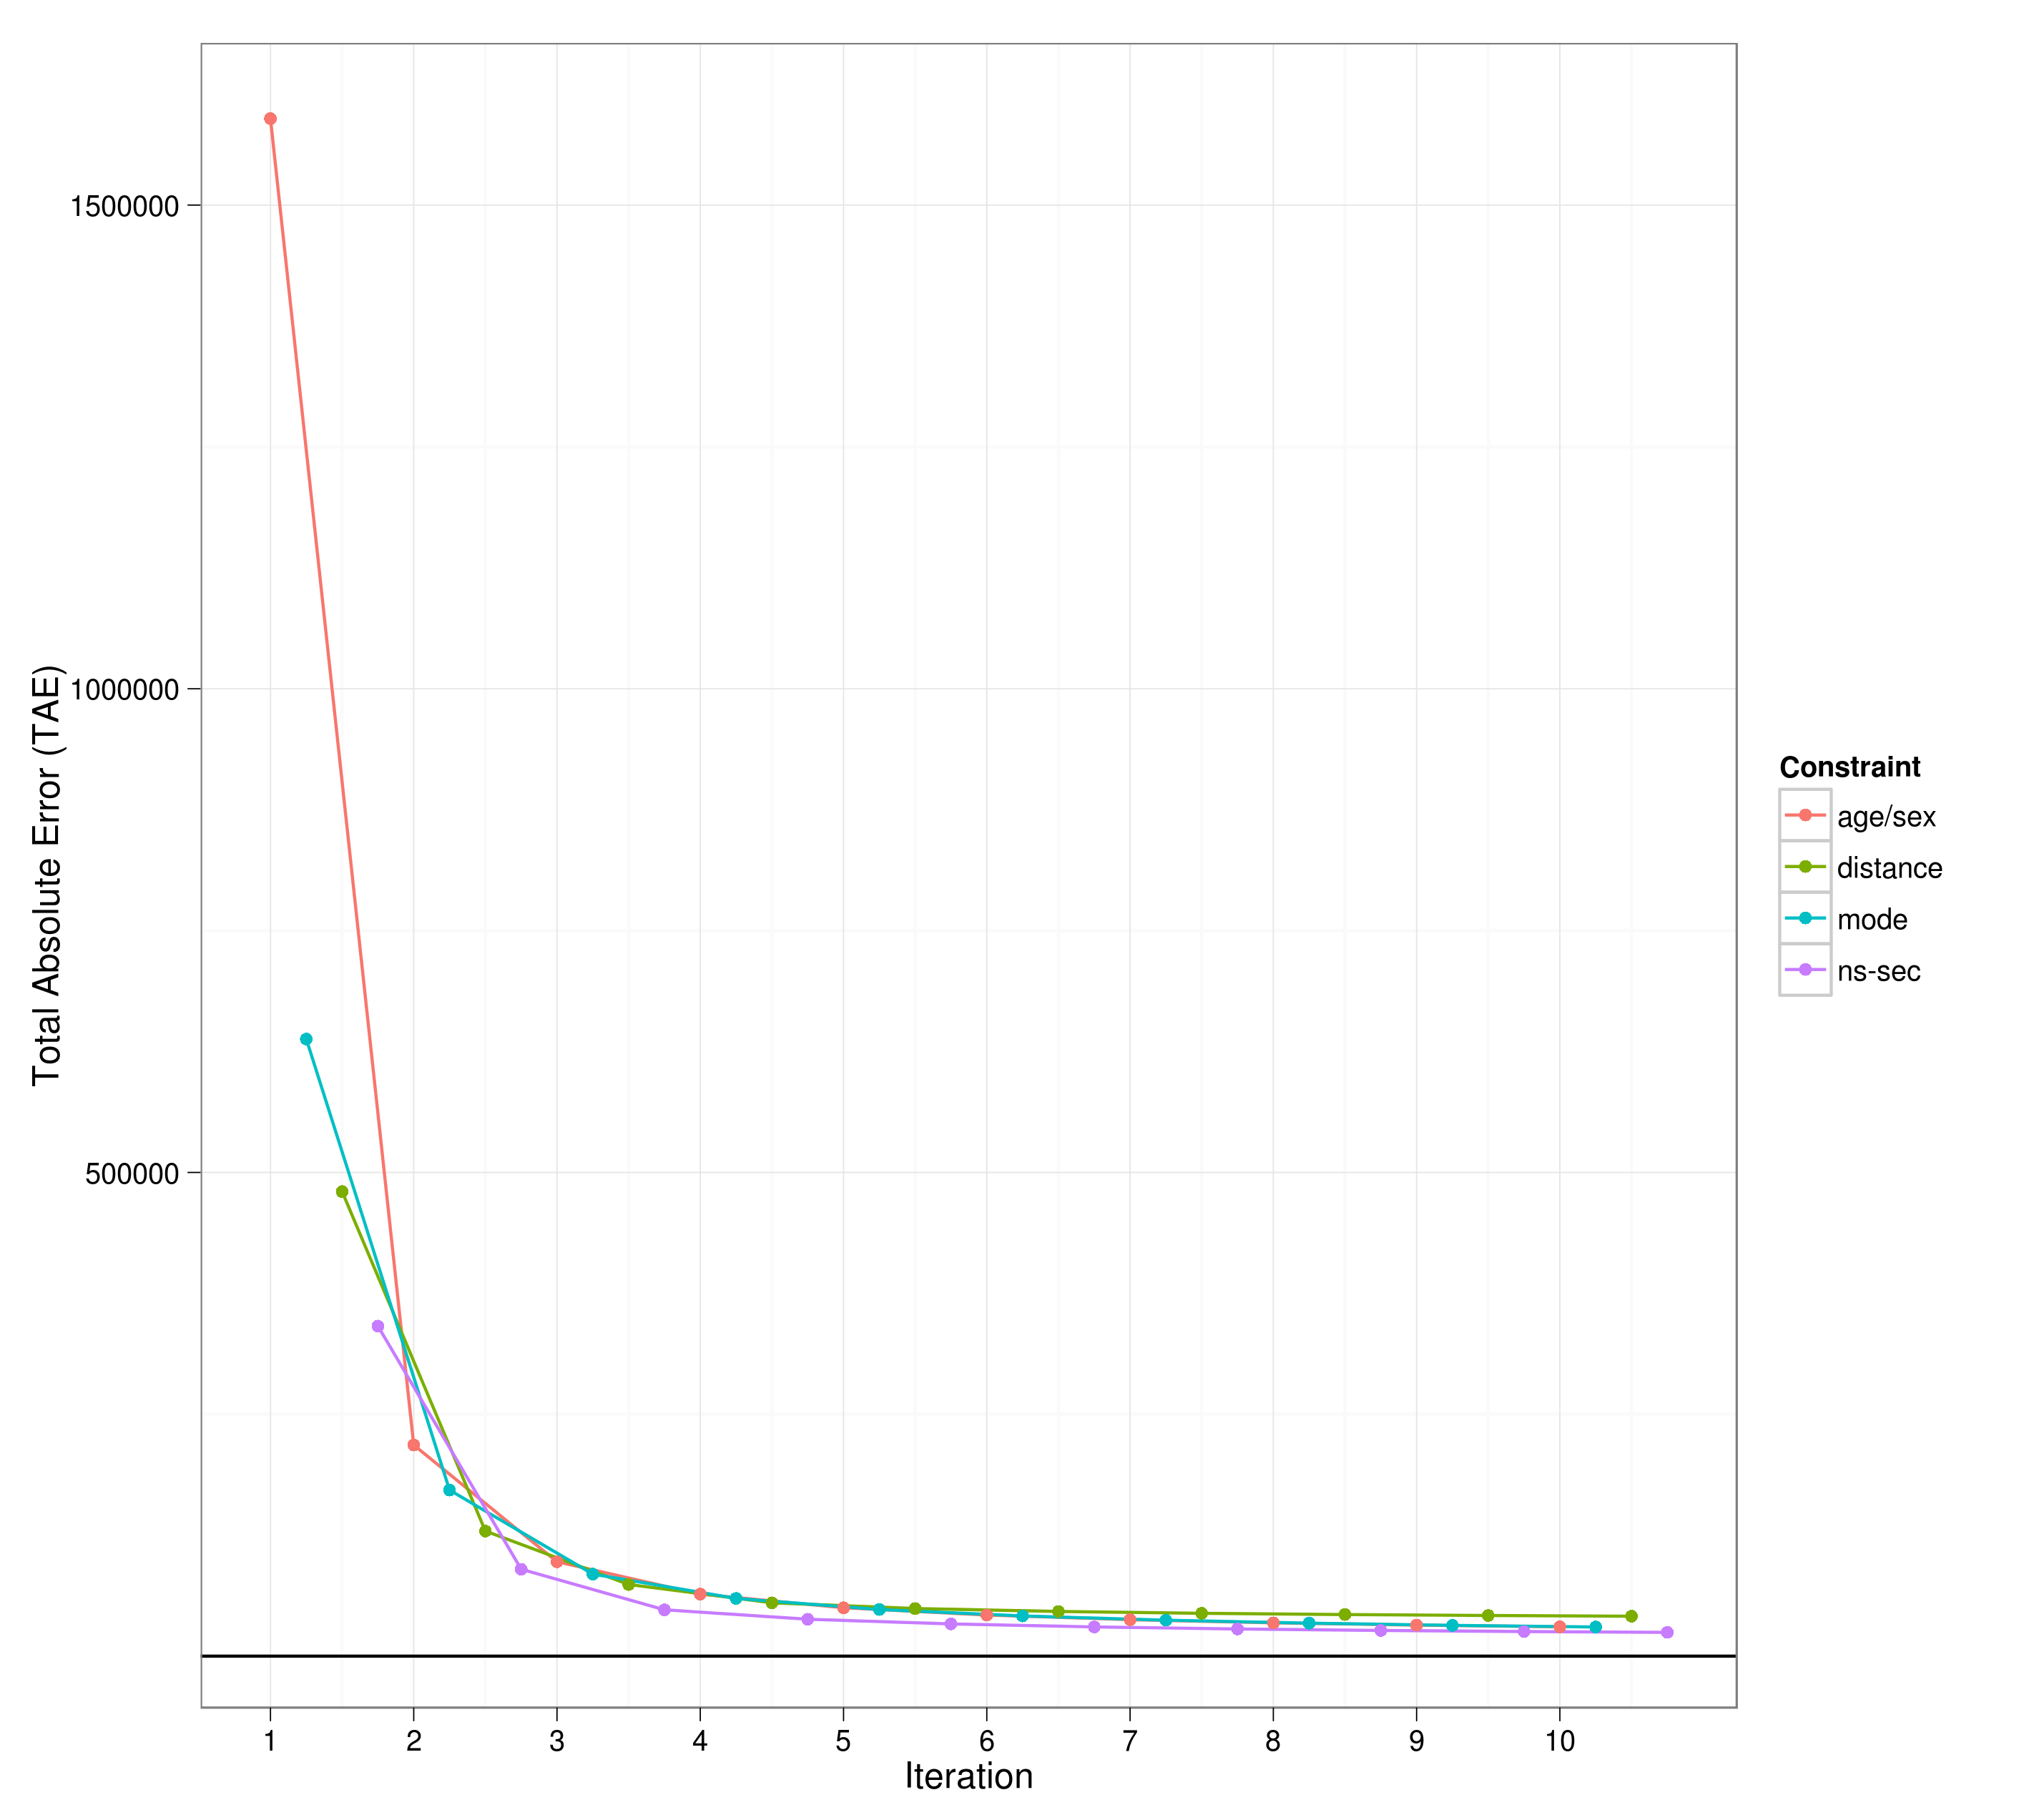
\includegraphics[width = 6.5 cm]{tae-it-plot}
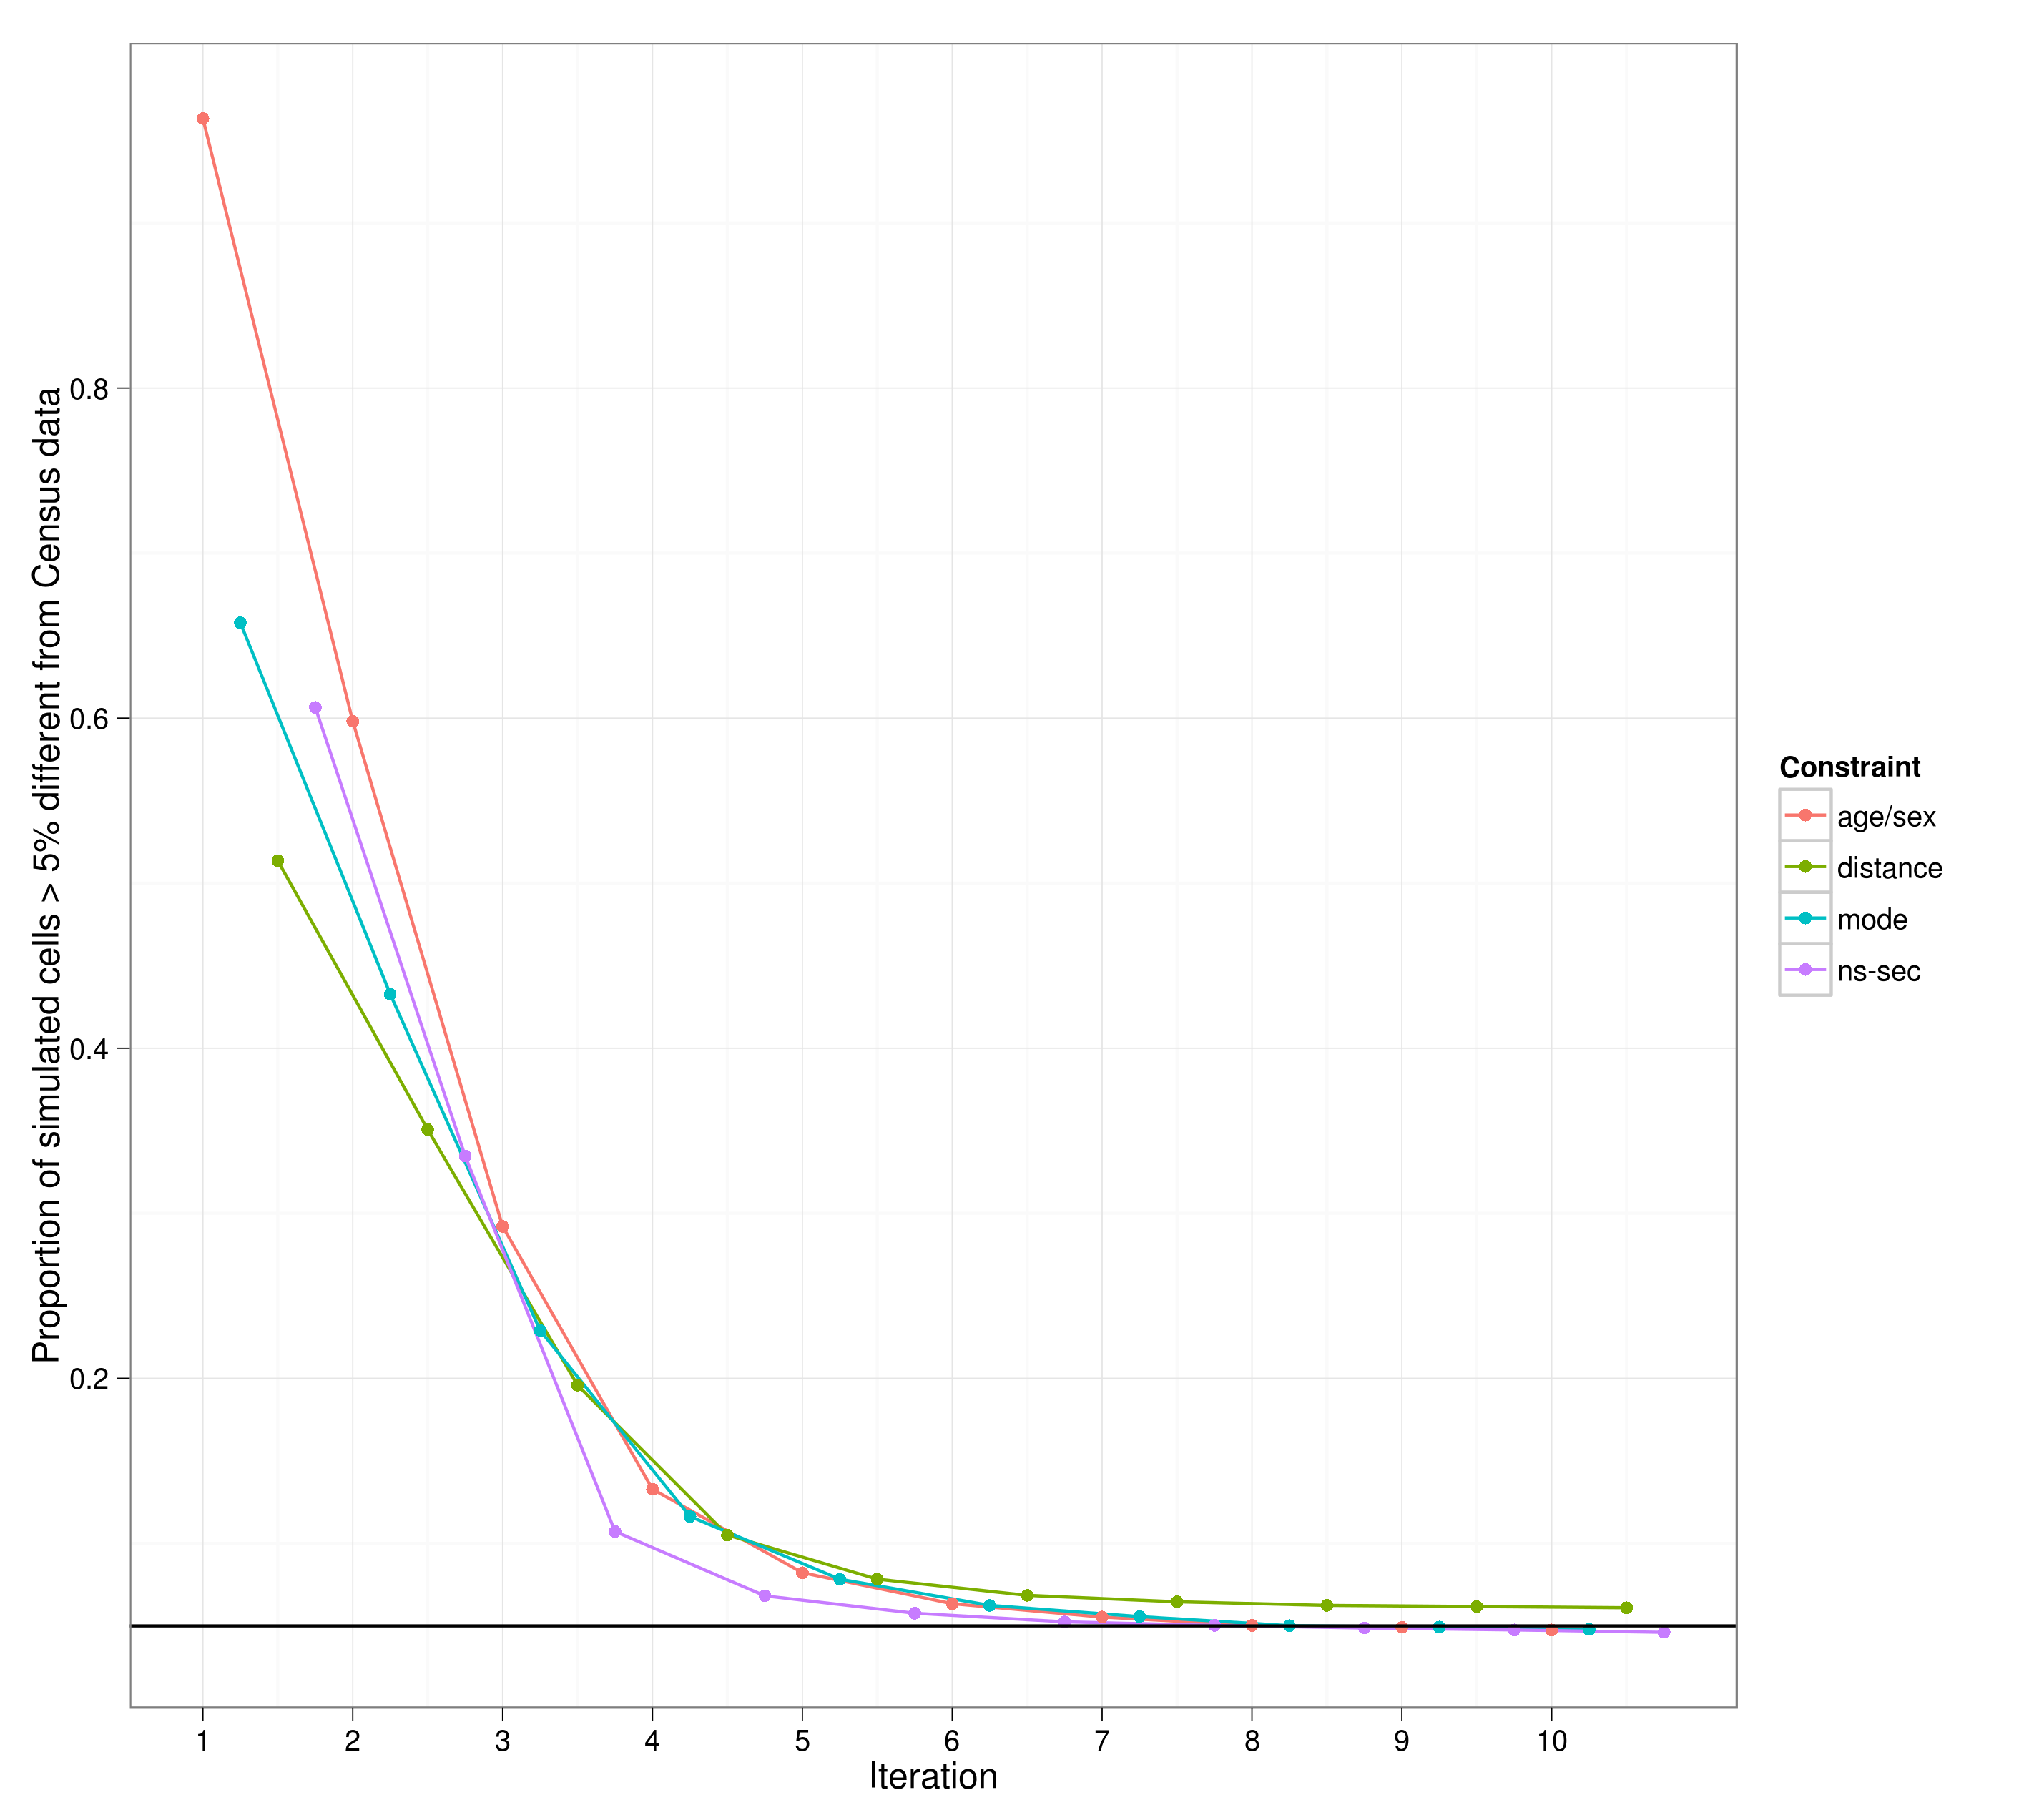
\includegraphics[width = 6.5 cm]{perc-it-plot}
\caption[Fit between simulated and census data]
{Improving fit between simulated and census data across all 4 constraint
variables outlined in \cref{Chapter4}, as illustrated by decreasing values of
the total absolute error (TAE) (left) and decreases in the proportion of
simulated aggregate cell values that differ from census data by more than 5\%
(right) after each constraint and iteration. The horizontal black lines
represent 0 error and 5\% of cell values, respectively. }
\label{f:fit-plot}
\end{figure}

The weighted data provided by IPF-based spatial microsimulation is bulky
(containing rows even for individuals who contribute very little: whose
weight is close to zero), making many types of analysis more difficult
(e.g.~contingency tables and~Gini Lorenz curves). To tackle
this problem, and provide a single
dataset for analysis using various techniques (e.g.~individual level,
geographic, or agent-based methods), the `truncate, replicate, sample' method
of integerisation was used \citet{Lovelace2013-trs}. Still, the final output
dataset contained 532,130 rows, representing every commuter in South Yorkshire.

\section{Assigning work location}
\label{s:workdes}
%  Original intro: weak
% What is the spatial distribution of energy intensive commuter patterns? What
% types of places are conducive to low-energy modes such as walking and cycling?
% Intuition would suggest an urban-rural divide, and that transport
% infrastructure would influence commuter patterns over space.
% This subsection provides more rigorous methods to investigate the spatial
% correlates of energy intensive commuter patterns.
The spatial microsimulation model results in a large dataset containing
hundreds of individuals for each zone under investigation. For micro level
spatial analysis, origin-destination pairs are needed: simulated
places of home and work need to be geotagged. The simplest solution
to this problem is to allocate all individuals in each zone home coordinates
corresponding to the zone's population-weighted centroid. Likewise, work coordinates
can be set to the nearest employment centre. This method allows
for simple analyses such as the proxy for geographic
isolation presented in Fig.~\ref{fig:dis-msoa}.

Rather than assuming that work centres are always located in the city
centre, a more realistic approach is to acknowledge that a variety of
employment centres exist, and that the relative importance of each varies from
place to place. This is illustrated in Fig.~\ref{fig:sflow}, a ward level
flow diagram of
the work locations of commuters based on the outskirts of Sheffield. Although
Barnsley is the closest city centre to Stocksbridge (see
Fig.~\ref{fig:dis-msoa}), this analysis makes it clear that Sheffield is the
primary non-home workplace.

\begin{figure}
\centering{
 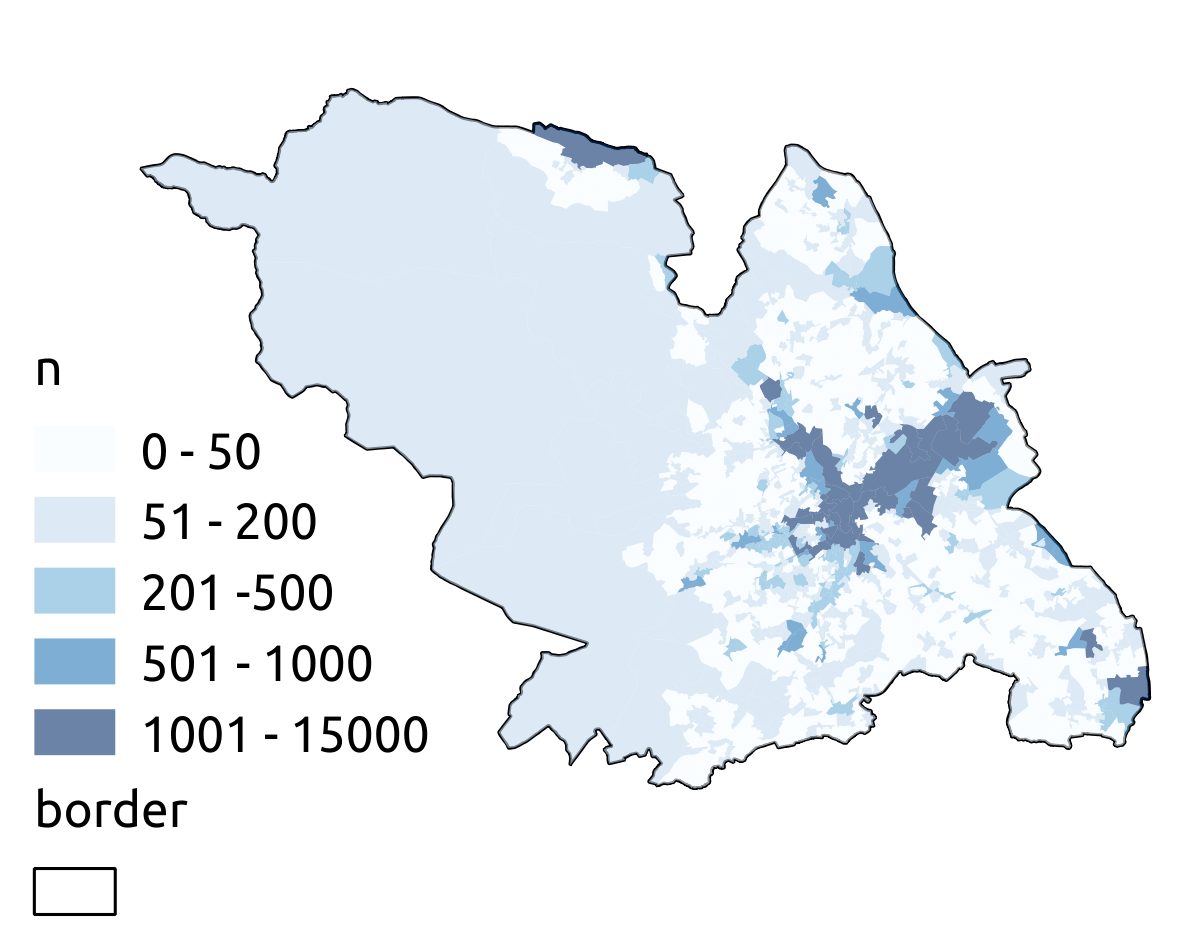
\includegraphics[width = 10 cm]{qgis-image-small}}
\caption[Employment density at the local level in Sheffield]
{Employment density at the local level in Sheffield (n is the number of
employees registered to each zone). These results
were generated by summing all incoming flows to all of Sheffield's 1,744
Output Area (OA) administrative zones. Data provided on a CD, on request from
http://www.nomisweb.co.uk/ .}
\label{fig:sworkdens}
\end{figure}
At an even finer geographical level, it is possible to discern the localities
within each city and ward where people are most likely to work based on UK
census data. This is illustrated in Fig.~\ref{fig:sworkdens}. Although this
level of geographic detail was not used in the final
results due to aggregation
issues,\footnote{The
Output Area flow data presented in \ref{fig:sworkdens} is difficult
to work with for individuals allocated to specific zones, because any
number between 1 and 4 is randomly set as either 0 or 3. This makes
the flow data essentially probabilistic for single Output Area pairs,
hence our limitation to aggregate level analysis of this dataset here.
}
it demonstrates the potential for highly localised work allocation based on
census-derived flow data.

\begin{figure}
\centering{
 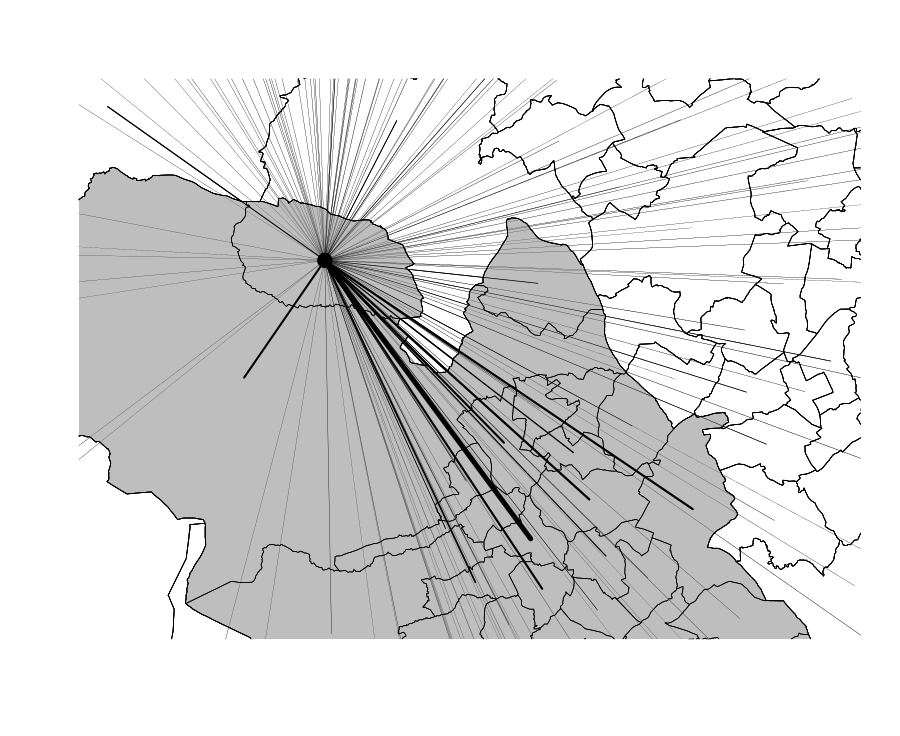
\includegraphics[width = 10 cm]{sflows}}
\caption[Flow diagram of commuter destinations from Stocksbridge]
{Flow diagram illustrating popular commuter destinations for citizens
of Stocksbridge. The thickness of the lines is proportional to the number of
people who travel there (for reference, 661 people travel to
the centre of Sheffield --- illustrated by the thickest line ---
and 2036 people work in Stocksbridge --- illustrated by the dot
from which all lines radiate. n = 6,338).}
\label{fig:sflow}
\end{figure}

The analyses presented in both Fig.~\ref{fig:dis-msoa} and Fig.~\ref{fig:sflow}
both greatly oversimplify trip routes. The straight lines underestimate travel
distance, completely ignoring the transport network. A more
realistic method is to randomly allocate each individual to a unique home
location based on
% data on houses, and work
% locations based on commuter flow data and the distance they travel to work
population density (or, potentially, local area classification) and estimate
the route taken using shortest trip algorithms dependent on the mode of
transport used (Fig.~\ref{fig:agent}). This latter method allows for the
calculation of route distances by mode, but is more complex and difficult to
implement over large areas.
%\footnote{?}

%%% This section is completely out of place...
% The results of spatial microsimulation include both continuous and
% categorical variables, posing a visualisation challenge during spatial
% analysis. Energy use, for example, depends on mode and distance travelled, so
% both variables should be seen together. Driving is the most popular form
% of commuting in all areas. Instead, the second most popular form of
% travel --- or lack of travel for those who work mainly from home (MFH) ---
% can be used to indicate variability in mode choice (Table \ref{t:cont}).

% \begin{figure}
%  \includegraphics[width = 13 cm]{map-lines-mode-dis}
% \caption{Second most popular mode of transport and average distance travelled
% for MSOA zones in South Yorkshire (add transport infrastructure and
% settlements).}
% \label{fig:dis-mode}
% \end{figure}
\begin{table}[htbp]
\caption[The 2nd most common mode of commuting compared with other factors]
{Contingency table illustrating the link between 2nd most common mode of
TTW in an area and average values for other variables.}
\begin{center}
\begin{tabular}{lrrrrr}
\toprule
2nd mode & \multicolumn{1}{l}{N. zones} & \multicolumn{1}{l}{Total (\%)} &
\multicolumn{1}{l}{$\overline{D}$ (km) } &
\multicolumn{1}{l}{$\overline{P}car$ (\%)} &
\multicolumn{1}{l}{$\overline{D}ens$ (People/km$^2$)} \\
\midrule
MFH & 18 & 10 & 17.0 & 68 & 31 \\ 
Tram & 4 & 2 & 10.8 & 53 & 179 \\ 
Bus & 95 & 55 & 11.2 & 54 & 106 \\ 
Car (p) & 10 & 6 & 13.5 & 63 & 40 \\ 
Foot & 46 & 27 & 13.2 & 53 & 112 \\
\bottomrule
\end{tabular}\end{center}
\label{t:cont}
\end{table}

These methods of spatial analysis provide great insight into the meaning of
aggregate statistics for groups of individuals at the city level of policy
intervention. However, to gain insight into the impacts of schemes on
individuals and local communities, agent based models may be needed.
In particular, there is great potential to link the work
presented here with relevant agent-based simulation work in the social
sciences (e.g.~\citealp{Gilbert2005a, Gilbert2007}) and
attempts to add a geographical dimension to this work
(see \citealp{Wu2008}).

To this
end Fig.~\ref{fig:agent} presents the simulated route choice of the 18
commuters selected from the spatial microsimulation model, and
contains both socio-demographic and geographic
detail.\footnote{For
example, the simulated car passenger who commutes to
central Sheffield in Fig.~\ref{fig:agent} is 16 years old, is classified as
class `other', and lives in a family that has access to 5 cars. These, and
further simulated details such as income, could, once validated, contribute
towards transport interventions targeting specific commuter groups.
}
% \footnote{This analysis results from 20 randomly selected
% individuals (2 of
% whom worked at home) from the spatial microsimulation model output for
% Stocksbridge and allocated origin-destination points based on known distance
% bands, ward-ward commuter flows, and the population density distribution of
% Stocksbridge.
% }
\begin{figure}
 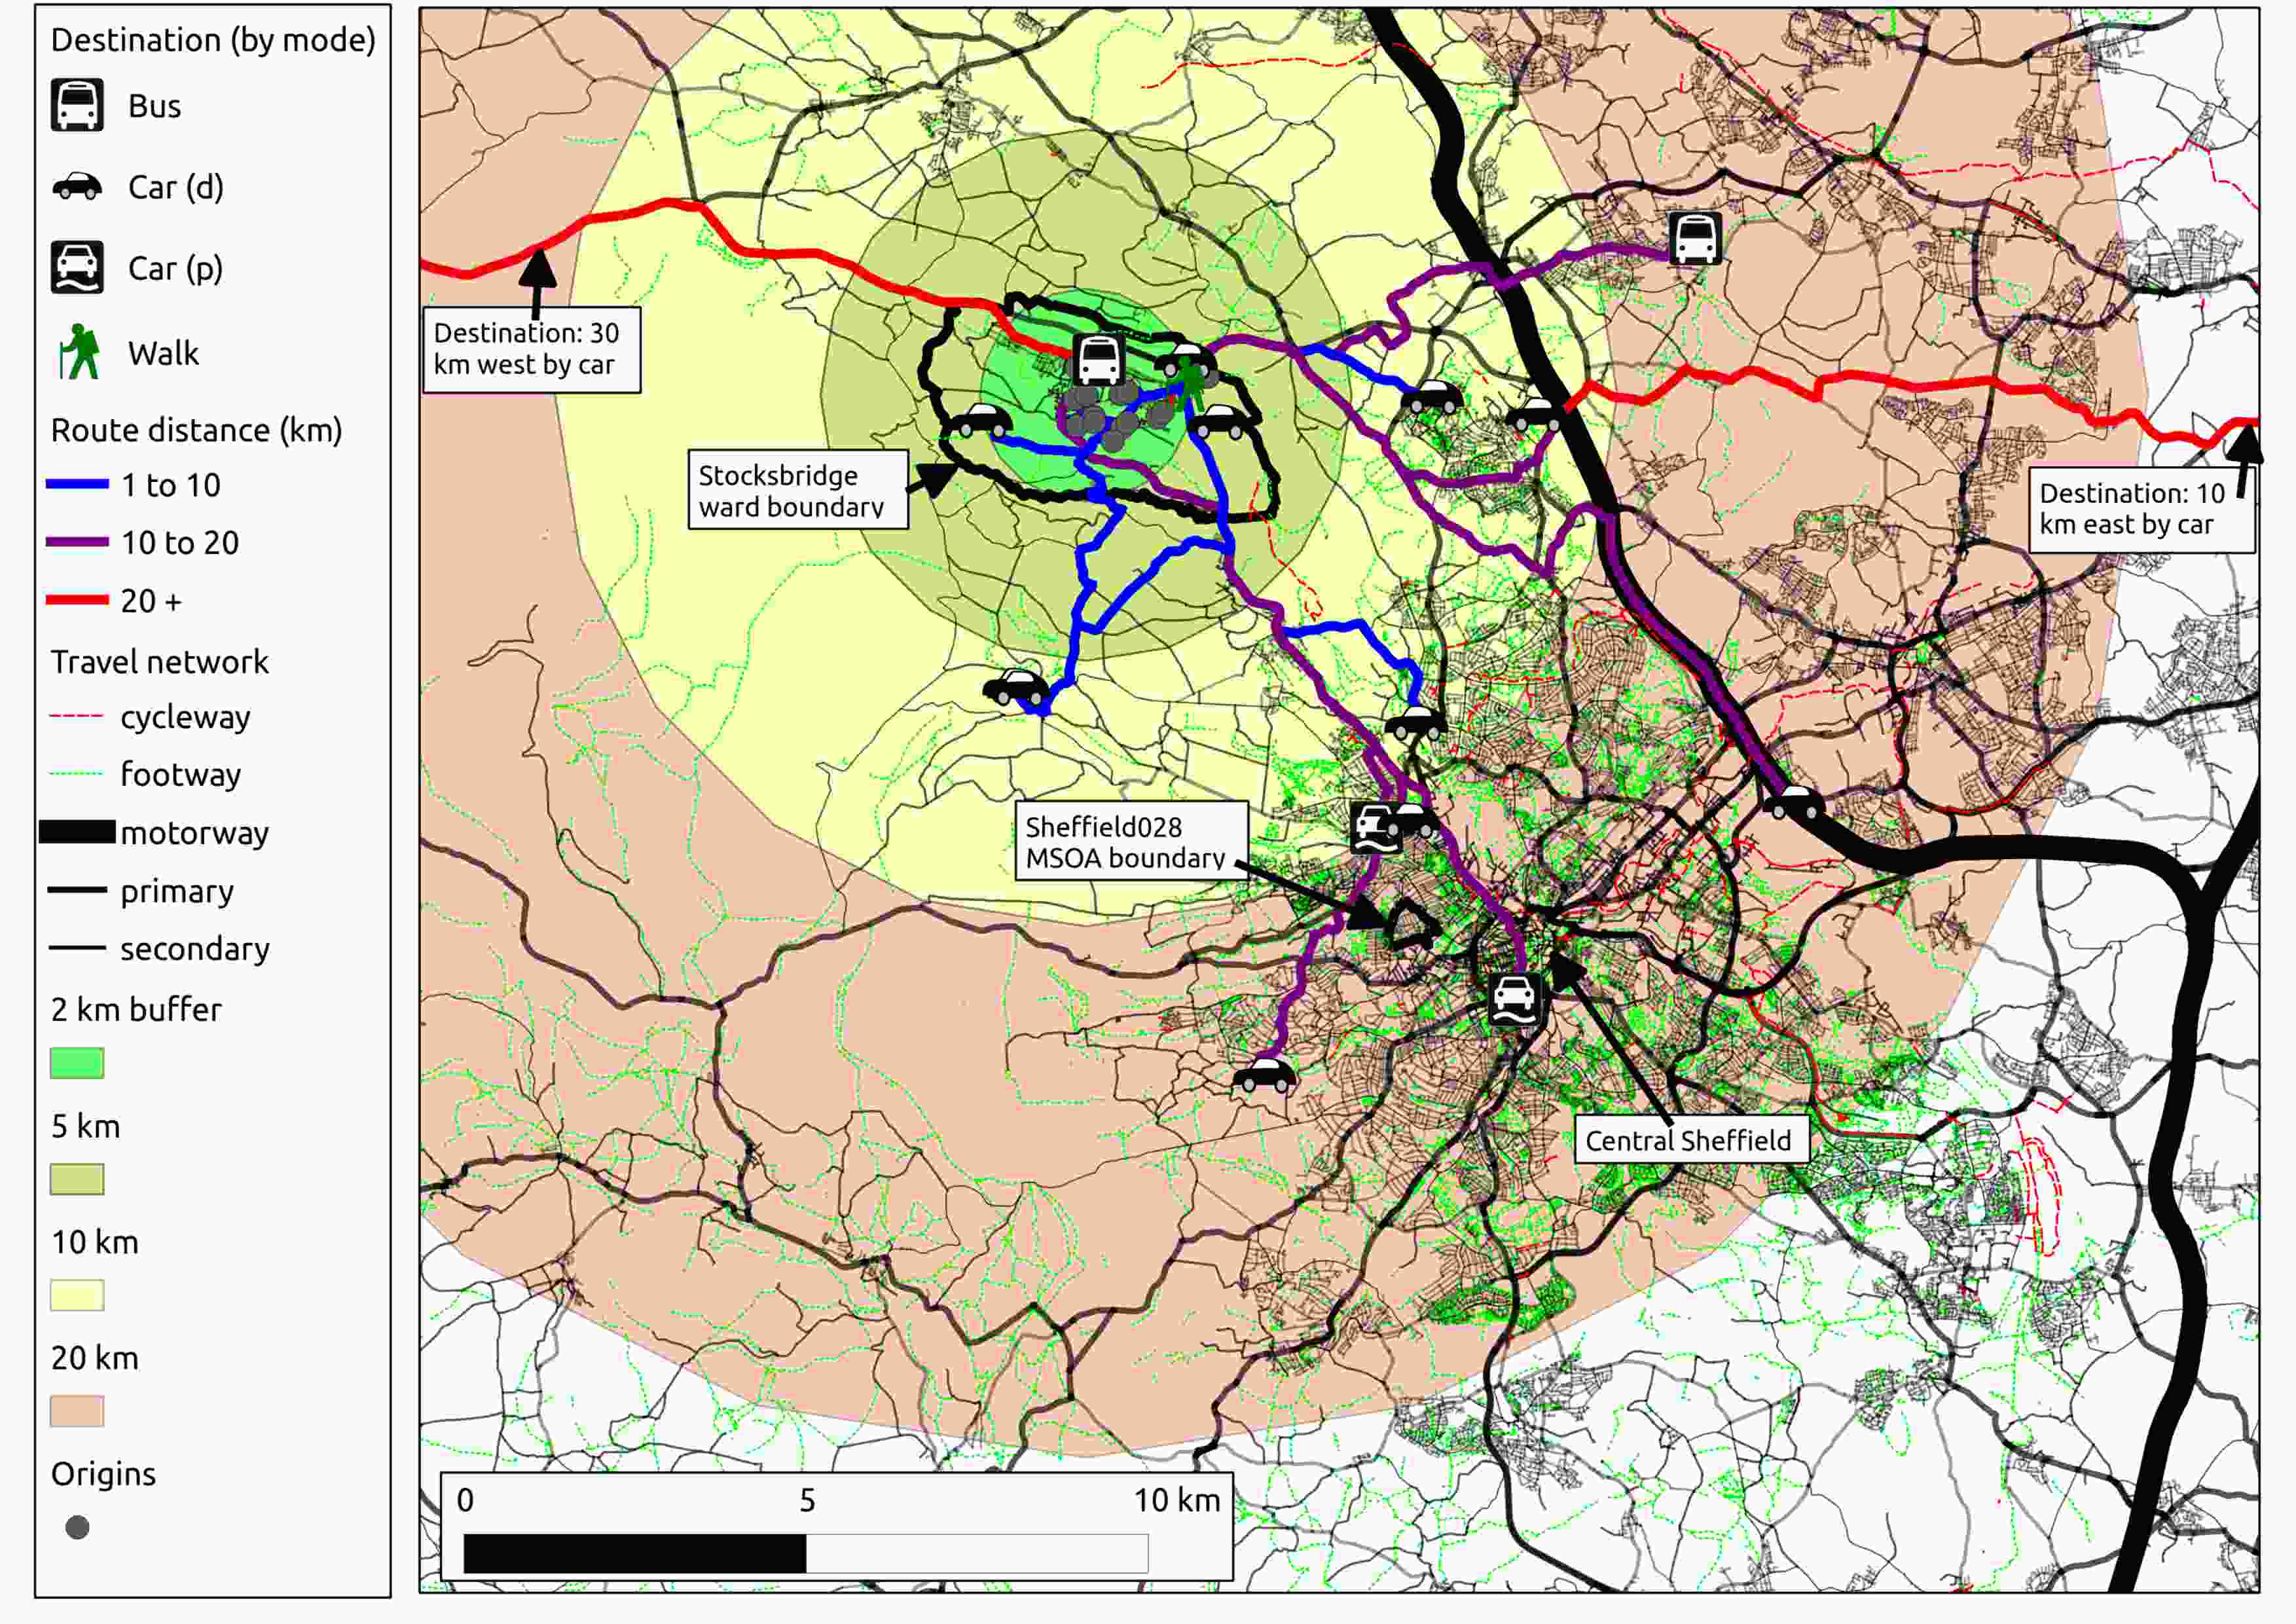
\includegraphics[width = 13 cm]{agents4}
\caption[Simulated route choice for 20 randomly selected individuals]
{Simulated route choice for 20 randomly selected individuals
from the spatial simulation model. Destinations were determined by 1) subsetting
destination wards by distance from Stocksbridge centre, 2) assigning
probabilities of working in each ward for each distance band (based on flow
data presented in Fig.~\ref{fig:sflow}) and 3) randomly selecting points
within the resulting destination wards. (Workplaces of 3 people who work from
home are not mapped).}
\label{fig:agent}
\end{figure}

The distances travelled along the transport network are clearly substantially
further than represented by simple straight lines. This concept can be
defined formally as \emph{circuity}, the ratio of straight-line distance
to route distance \citep{Ballou2002}. Fig.~\ref{f:circ} illustrates the impact
of the road network on distance travelled. Overall, the route distance
represented in Fig.~\ref{fig:agent} is 223 km, 24\% further
 than the straight-line distance (179 km) for the 17 commutes. As in previous
studies, circuity tends to decrease approximately logarithmically as a function
of distance \citep{Levinson2009}. The spatial microsimulation method holds
great potential for investigating the impact of the travel network, especially
when combined with new tools for batch-processing of shortest-route
algorithms.\footnote{The
analysis conducted one trip at a time, using the
QGIS plugin ``Road Path'' for a simple solution with a user-friendly interface.
(\href{http://docs.qgis.org/2.0/html/en/docs/user_manual/plugins/plugins_road_graph.html}
{http://plugins.qgis.org/} ).
To automate the process, Routino (http://www.routino.org/), PGRouting
(http://pgrouting.org/) or the recently released R package osmar
(http://cran.r-project.org/web/packages/osm) could be used.
The rapid evolution of transport network data and software
provides avenues for methodological advance.
}
\begin{figure}
\begin{center}
 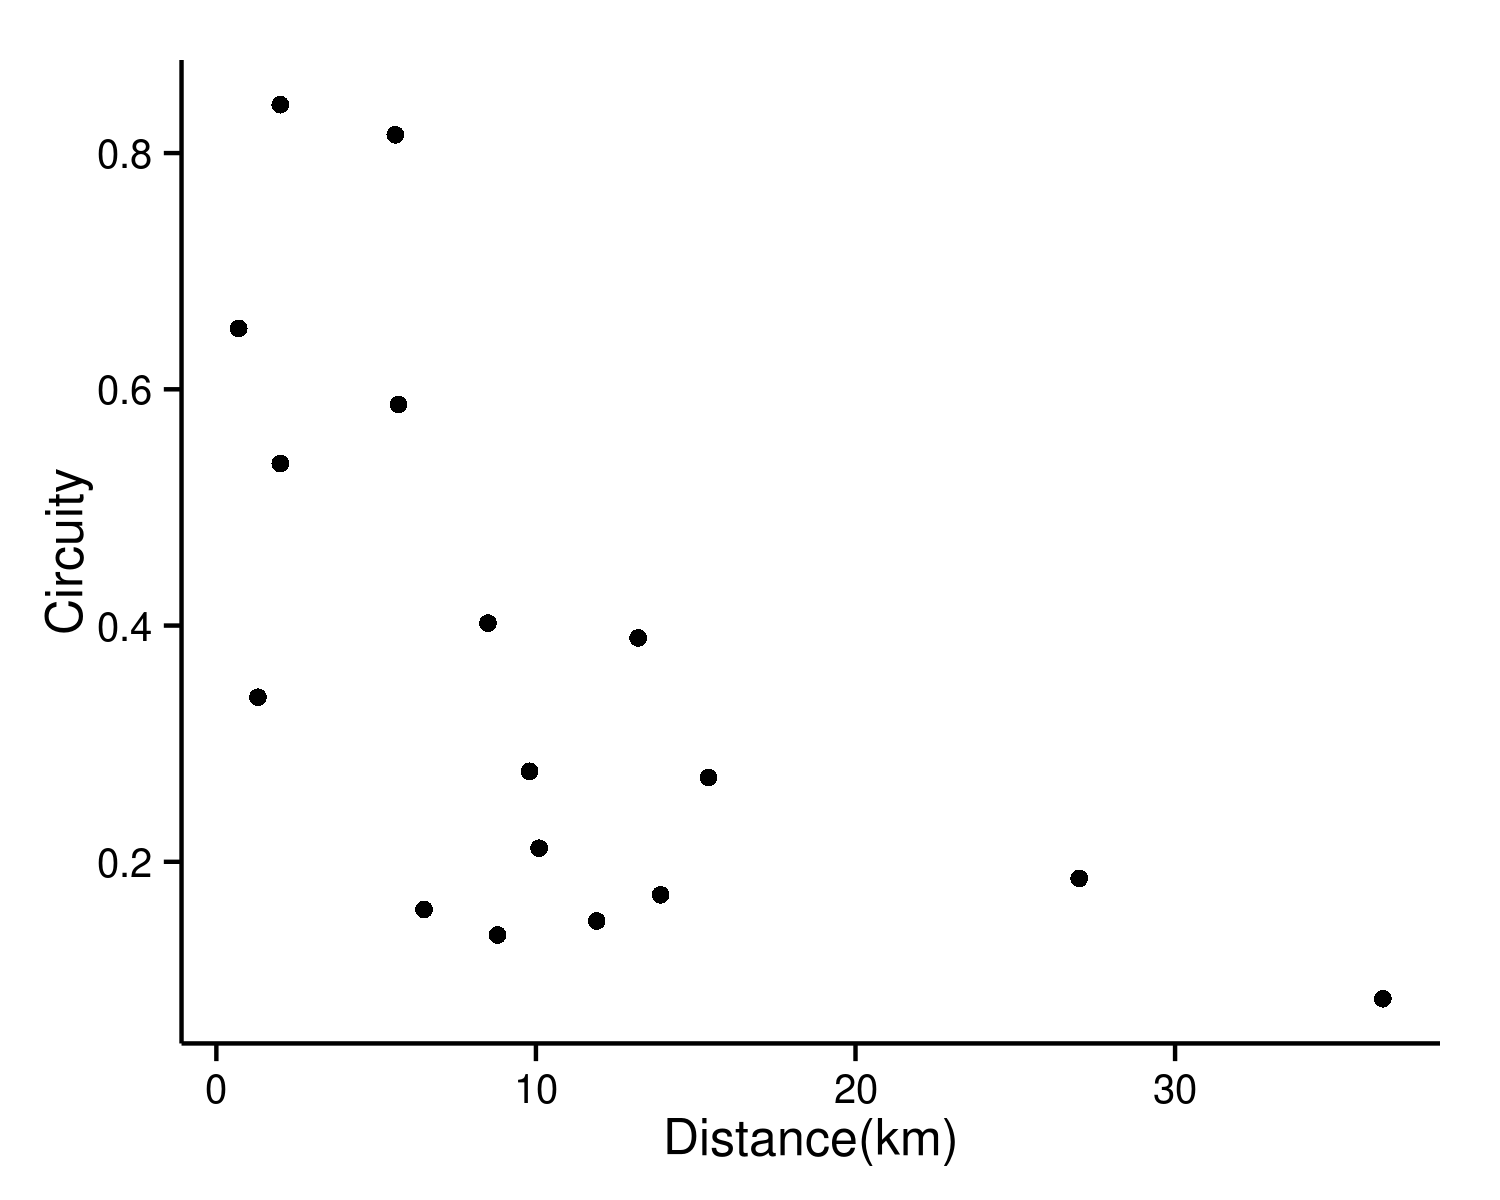
\includegraphics[width = 8 cm]{cirqui17}\end{center}
\caption[Circuity as a function of distance in Sheffield]
{The circuity of the route distance as a function of the
straight-line distance for 17 commuter trips modelled in Stocksbridge.}
\label{f:circ}
\end{figure}

\section{Model validation} \label{s:valid}
% % Internal vs external validity; comparison
Due to the dangers of using incorrect model data to inform policy,
the importance of validation has been emphasised repeatedly in the
spatial microsimulation literature \citep{Holm1987, chin2006regional,
Smith2009,Clarke2010-valid, Ballas2013-4policy-analysis}.
Because the outputs of spatial microsimulation
are by nature detailed and provided at the individual level, validation
is challenging: ``such detailed information is virtually never
available at the disaggregate level for an entire region''
\citep[p.~37]{Ravulaparthy2011}. In fact, one could argue that
if individual microdata were made available at the small area level,
spatial microsimulation would be obsolete.

Researchers using spatial microsimulation have been innovative at
overcoming this `catch 22' situation, using a variety of methods.
In broad terms, there are two types of strategy available:
internal and external validation \citep{edwards2013validation}.
The first of this is relatively
straightforward: the aggregated constraint variables are compared with the
aggregated results of the spatial microsimulation model for the same variables.
In our model, the results of this test were reassuring: the correlation between the
aggregate counts from the census and those generated in our spatial microsimulation
were 0.9989 overall for all 6,920 data points (40 categories by 173 zones).
However, the quality of the fit was better for some constraint variables than
for others: the r$^2$ values for the distance and mode variables were
0.9993 and 0.9983, primarily due to the inaccuracy or our estimates of
individuals who work mainly from home (mfh) (Fig.~\ref{finvalid}).


\begin{figure} \begin{center}
    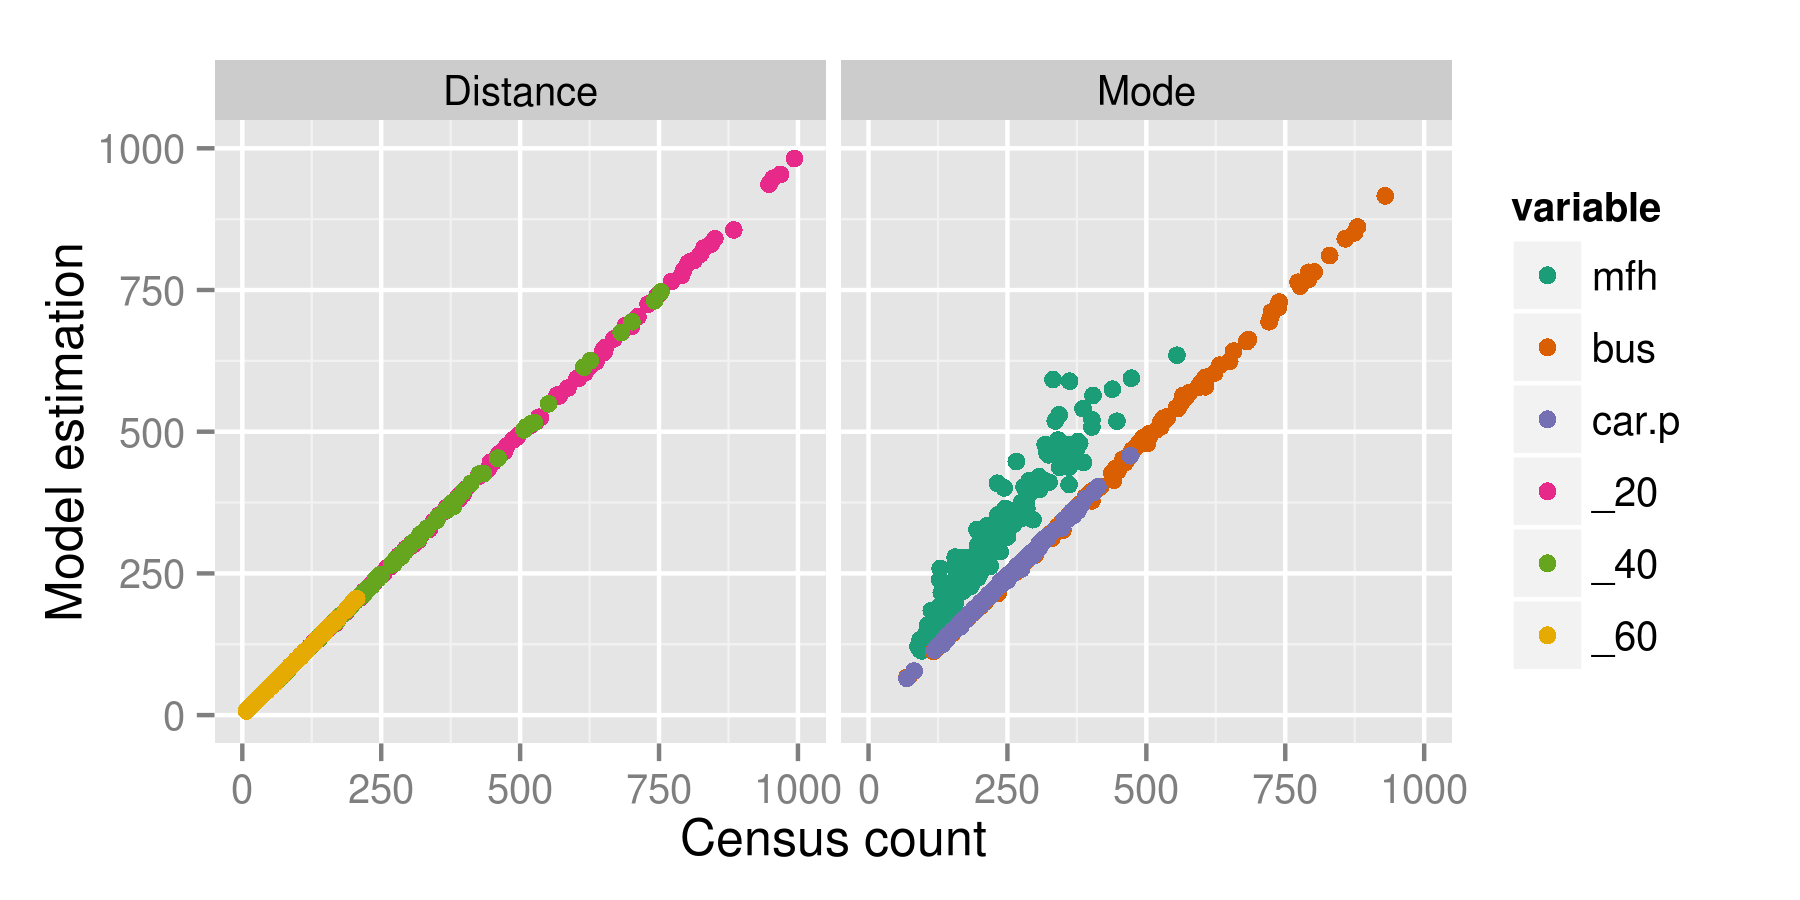
\includegraphics[width=12cm]{invalid}
 \end{center}
 \caption[Comparison of census and simulated results at the aggregate level]
 {Comparison of census and simulated results at the aggregate level
 for a selection of six categories from the mode and distance constraints.
 The 20 category, for example, refers to the number of people travelling
 10 to 20 km to work.} \label{finvalid}
\end{figure}


This internal validation
result is less impressive when one considers that IPF always converges
towards the optimal result for known constraint variables:
it is the unknown cross-tabulations and
target variables that are the most useful result,
so external validation should, in many cases, be the focus
\citep{Morrissey2008, edwards2013validation}.
Four methods of corroborating spatial microsimulation results with external
data were identified:
\begin{itemize}
 \item Compare simulation results with real spatial microdata.\footnote{Income,
for example, is collected by the Census, but is not disseminated at aggregate
levels, let alone the individual level geocoded data required to validate the
individual level results of the spatial microsimulation model. Access to such
sensitive real microdata limits the applicability of this method.}
\item Collect primary data from specific areas against which the simulated
results can be tested.\footnote{In some cases (e.g.~environmental attitudes)
this may be the only reliable validation option, as the data is simply not
collected in geo-coded surveys.}
\item Compare simulation results at the aggregate level with estimates
from a dataset external to the model \citep{Morrissey2013}.
\item Aggregate-up the small area estimates provided by spatial microsimulation
to compare the results with real data that \emph{is} provided at higher
geographies \citep{Edwards2009}.
% \footnote{To provide another example,
% domestic energy use, which is provided in the Understanding Society
% dataset, is disseminated at the
% LA level by the Department of Energy and Climate Change (Decc), which
% constitute 40 to 50 Medium Super Output Areas (MSOA) combined.}
% \item Compare aggregate level results of the model with census variables that
% were not constrained for. % Include this if needs be, or in thesis.
\end{itemize}
Each of these options was considered for our case study,
but data constraints meant that only one, comparison of aggregate data
on a target variable with a reliable external dataset, was deemed viable.
The target variable chosen for this was income; Neighbourhood Statistics
provides estimates of this at the MSOA level, allowing
for direct comparison with our results (Fig.~\ref{fincome-scatter}). The results show
high levels of correlation ($r^2 = 0.93$) between simulated incomes and official
estimates, although the spread of the values resulting from spatial microsimulation
underestimated the true level of inter-zone variation in average incomes.

\begin{figure}[h*]
 \centering
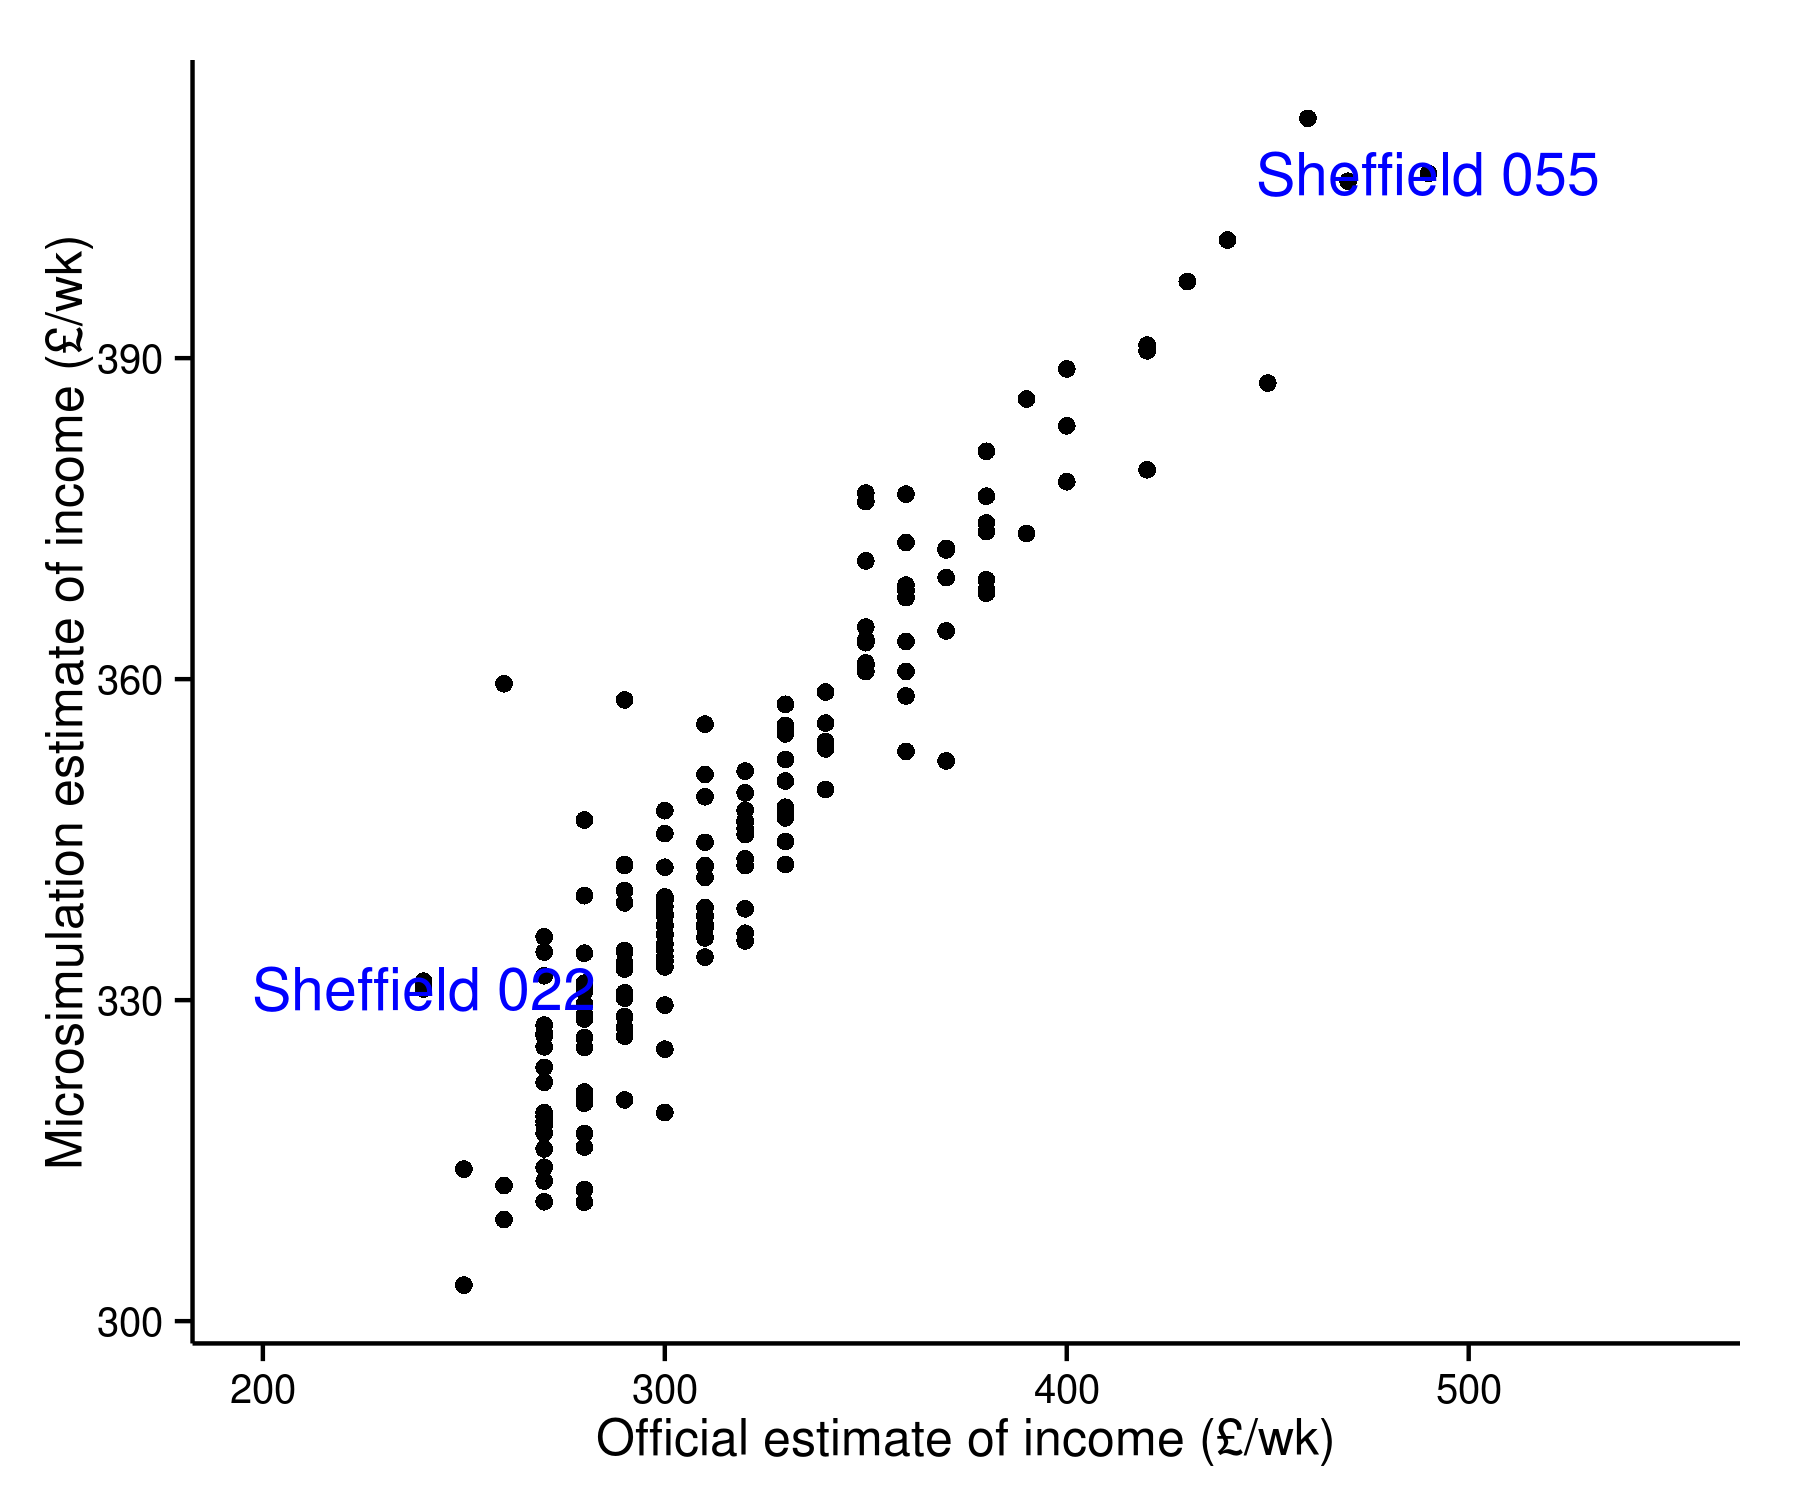
\includegraphics[width=13.5cm]{income-scatter}
 \caption[Mean equivalised household income from official and simulated data]
 {Scatter graph of mean equivalised household income produced as an
 output from the spatial microsimulation model (y axis) and official estimates
 from the Office of National Statistics for the 173 Medium Super Output Areas
 of South Yorkshire. Maximum and minimum official estimates labelled in blue.}
 \label{fincome-scatter}
\end{figure}

\section{Results} \label{c7results}
The results show that, at the aggregate level, South Yorkshire's commuting
behaviour is comparable to the national average. Nevertheless, the
microdata illustrate substantial
inter- and intra- zone variability. Table \ref{t:sum} illustrates the
cross-tabulations (contingency tables) that are made possible
when spatial microdata are used. Univariate statistics are available on
mode of transport, age and number of cars but the interaction between these
variables remains hidden in aggregated Census data.

\begin{table}[h]
\caption[Summary statistics of the commuting behaviour of in South Yorkshire]
{Summary statistics of the commuting behaviour of individuals in South
Yorkshire disaggregated by mode. (Motorbike, taxi, metro and `other'
modes have been removed for brevity).}
\begin{center}
\begin{tabular}{lrrrrrr}
\toprule
Mode & N.  & \%  & \% National & Age & Distance (km) &
Ncars \\
\midrule
Bus & 31486 & 7.2 & 7.4 & 38.3 & 7.5 & 0.5 \\ 
Car (d) & 268496 & 61.1 & 54.6 & 40.1 & 14.3 & 1.9 \\ 
Car (p) & 38233 & 8.7 & 5.9 & 33.5 & 14.5 & 1.5 \\ 
Cyc & 4498 & 1.0 & 2.6 & 38.3 & 5.0 & 1.1 \\ 
% Metro & 692 & 0.2 & 3.8 & 32.0 & 8.7 & 0.8 \\ \hline
MFH & 45326 & 10.3 & 9.3 & 40.0 & 0.0 & 1.9 \\
% Moto & 4844 & 1.1 & 1.1 & 37.0 & 11.0 & 1.3 \\ \hline
% Other & 692 & 0.2 & 0.5 & 42.8 & 8.8 & 1.5 \\ \hline
% Taxi & 1211 & 0.3 & 0.5 & 38.9 & 8.5 & 0.3 \\ \hline
Train & 5709 & 1.3 & 4.6 & 36.9 & 24.6 & 1.2 \\ 
Walk & 38406 & 8.7 & 9.7 & 36.6 & 3.1 & 0.8 \\ 
Average & - & - & - & 39.0 & 11.3 & 1.6 \\
\bottomrule
%%% sort out walking distance too!
\end{tabular}\end{center}
\label{t:sum}
\end{table}

Beyond illustrating the capability of spatial micrsimulation to provide
estimated cross-tabulations of aggregate level data,
Table \ref{t:sum} also provides substantive information
about commuting patterns that could be applied to transport policy:
\begin{itemize}
 \item Cars dominate travel to work in South Yorkshire, to an
even greater extent than in England as a whole.
\item The dominance of cars is even greater when measuring travel
to work in terms of distance travelled: car commuters travel on
average further than all other types of commuters bar those who commute
by train.
\item There are also substantial differences in the age profiles of
different commuting modes: walking, which is often associated with older
members of society, appears to be more prevalent amongst the young. Bicycle commuters,
who are sometimes stereotyped as young \citep{Daley2011}, are not much younger
than the average. Car drivers and home workers tend to be slightly older.
\item Car ownership, which is seldom factored into transport policy assessments,
\citep{Kay2011}
varies with the mode of travel to work. Those who catch the bus or walk are least
likely to own a car, while a those who drive to work or work from home own on
average almost 2 cars per household.
\end{itemize}


As in England as a whole, it is clear that cars, in round numbers, constitute
70\% of trips (61\% of commuters drive to work; 9\%
are passengers in other peoples' cars). The utility of the individual level
results is illustrated at this aggregate level by observing differences in
average age and distance of commute between modes: car drivers and bus
passengers are on average older than those who walk to work.
Unsurprisingly there are also differences in the average distance
travelled. Train passengers travel 13 km further than average;
those travelling by bus or non-motorised modes tend to live closer
to home.
A predictable, yet rarely investigated, result from Table \ref{t:sum},
is the high variability in the average number of cars in households of different
types of commuters: bus passengers appear to have the fewest cars per household
of all modes. Each model result has the potential to inform policy. The final one,
for example, provides support for the argument
 that public transport policies are currently failing to
 ``lure car users out of the car''
\citep[p.~193]{Davison2006}.\footnote{As
with the
other non-constrained variables target variables described in Table
\ref{t:indata}, this model result should be validated by additional data before
strong conclusions are drawn.}
% Cite the sdc article here !!!

From this, total distance travelled and
energy use by mode per year can be calculated.
Fig.~\ref{fig:proportions} presents these model
results (of which distance is most robust, as it is constrained by Census data)
for the average and range for all 694 MSOA zones in Yorkshire and the Humber.

\begin{figure}[h*]
 \centering
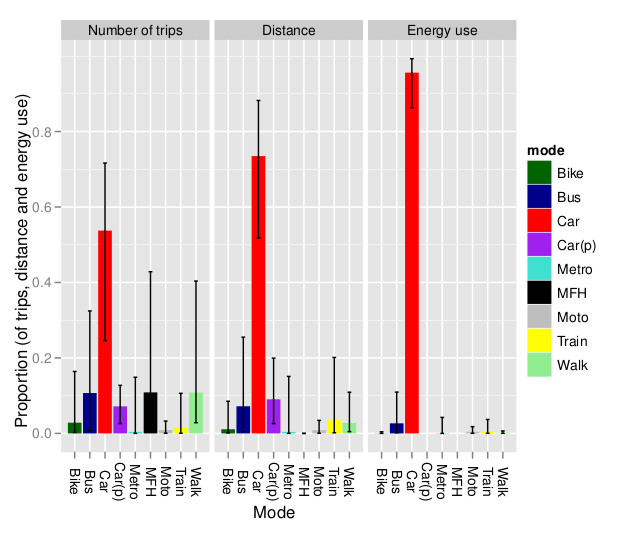
\includegraphics[width=10cm]{proportions}
 \caption[Proportion of trips, distance, and energy by mode]
 {Proportion of trips, distance, and energy use accounted for by
different commuter modes. The error bars represent the range of values within
MSOA areas in Yorkshire and the Humber.}
 \label{fig:proportions}
\end{figure}

The proportion of energy
used by cars for transport to work is 95.6\%: \emph{this is more than 20 times
the energy costs of all other modes of transport put together}.

An illustration of the increasing dominance of cars as one moves from trip
number, through distance travelled, and then energy use metrics, is provided in
Fig.~\ref{fig:proportions}. Note that in some regions car drivers account for
less than a third of all commuter trips. Yet in terms of energy use, cars
consume more than 85\% of all energy consumed for getting people to work and
back.

The results show a strong relationship between location and
 distance travelled.
The role of location, and distance to employment centres
more specifically as a cause of distant
commutes was explored using travel to work (TTW) zones, defined by the Office
for National Statistics at the wider regional level of Yorkshire and the Humber
(Fig.~\ref{fig:map1}).\footnote{The
wider regional level of analysis of
Yorkshire and the Humber (see Fig.~\ref{f:scales}) was used in this case
because TTW zones are large: only 3 are found in South Yorkshire
(Fig.~\ref{fig:dis-msoa}), so a larger area is useful to see the overall
pattern. Travel to work zones are defined as ``zones with a self- containment of
at least 75\% (which is to say that less than 25\% of those who work in an area
live outside it, and less than 25\% of the employed residents of that area
commute to workplaces outside the same area)'' \citep{Coombes1982}.
}
\begin{figure}[h]
 \centering
 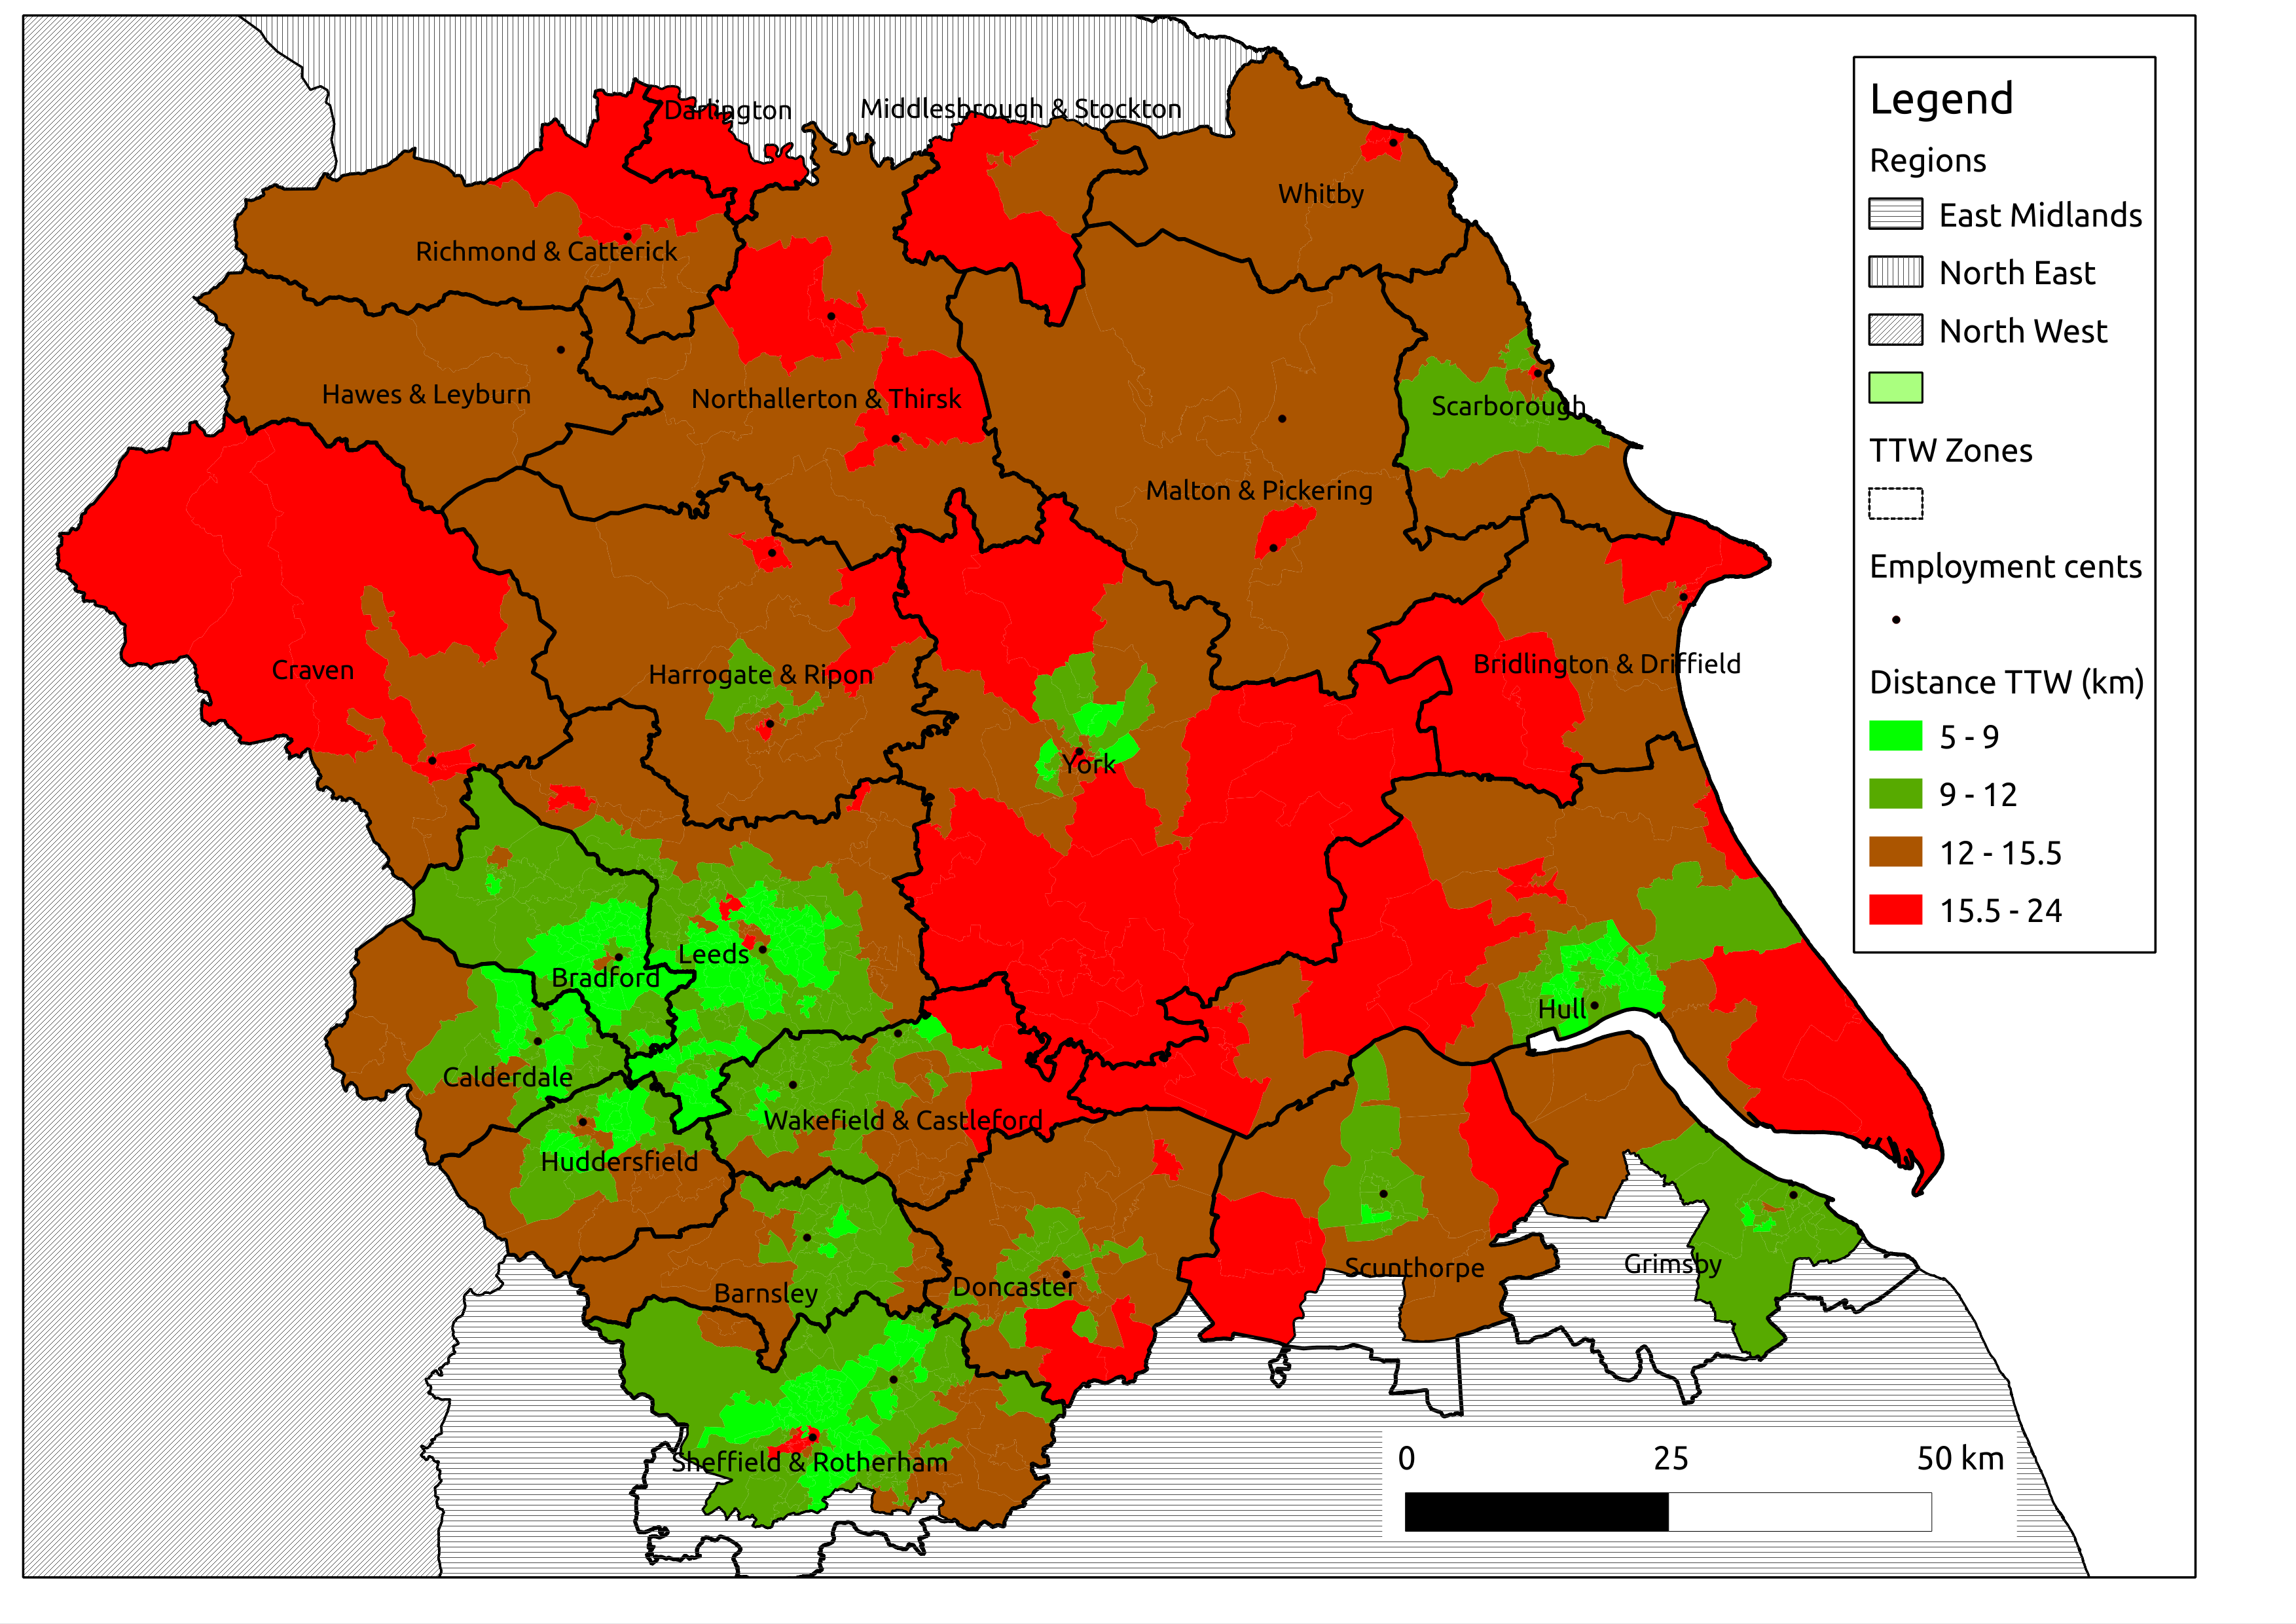
\includegraphics[width=14cm]{dismap2}
 \caption[Average distance travelled to work in Yorkshire and the Humber]
 {Average distance travelled to work in Yorkshire and the Humber by MSOA
zone. Black lines represent TTW zones.}
 \label{fig:map1}
\end{figure}
Fig.~\ref{fig:map1} shows that MSOA areas located in and
around the conurbations surrounding Bradford, Sheffield and Hull tend to have
low average commuter distances, while rural locations such as the North
York Moors are associated with long average commutes. This result differs
from that of suburban USA (where urban sprawl accounts for high commuting costs
even within major conurbations), but it is hardly new or surprising
\citep{Marshall2008, Sexton2011}.
An unexpected result is the tendency of city centres to be associated
with high average commuter distances. This can be seen in red patches surrounded
by a sea of green in the centres of Bradford, Leeds, Scarborough and Sheffield.
(One hypothesis to explain this is as follows: some city centres attract
wealthy individuals, who tend to commute further, often by train.)
Energy costs are directly proportional to distance travelled for all
modes. It is therefore unsurprising that average energy cost of commuter trips in each area
are closely related to the distance of commute (r = 0.97).
Distance is the most important driver of energy costs at the MSOA level within
Yorkshire and the Humber; the correlation between average distance and average
energy use per commuter trip is 0.97.
The
geographical causes of energy intensive commuting are therefore the same as the
causes of high average commuter distances at the MSOA level.

\begin{figure}
\begin{center}
  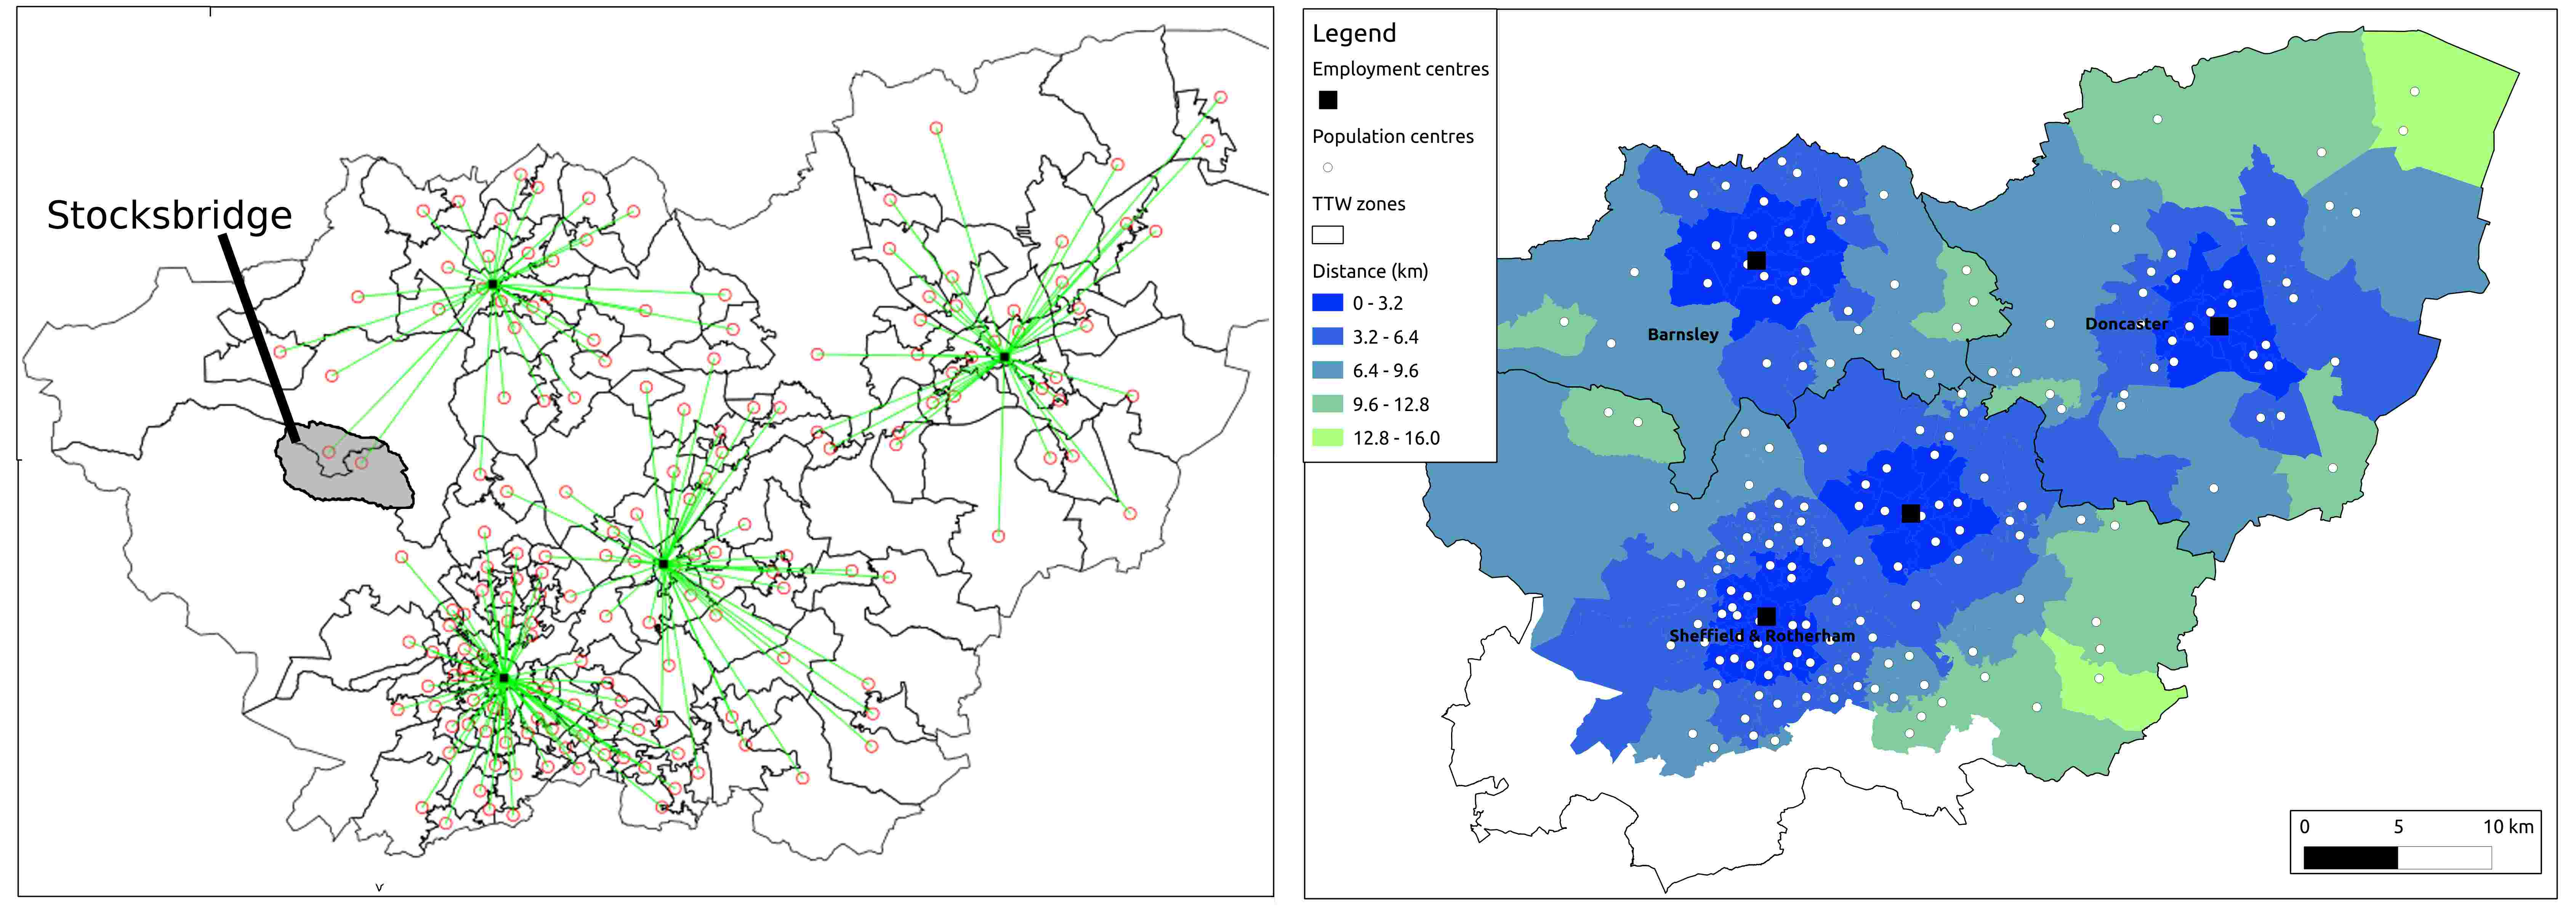
\includegraphics[width = 13 cm]{distances-msoa2}
\end{center}
\caption[Average distance to employment centre in South Yorkshire]{Average
distance to employment centre in South Yorkshire. The
left-hand map illustrates how distance was calculated (using the command
 nncross() in the R package `spatstat'). The right-hand map illustrates
the results --- Sheffield and Rotherham are grouped together in the same
travel to work zone.}
\label{fig:dis-msoa}
\end{figure}

To explore this link further, the average distance from employment
centre
was calculated (\ref{fig:dis-msoa})
and plotted against the average energy cost of transport to work in each MSOA,
see dots in Fig.~\ref{fig:dis-e}. The reversal of slope in the
tick-shaped curve of the relationship between distance to employment centre and
energy use suggests that the link between these variables is not as simple as
one might expect: other factors are at play, possibly linked to
individual level variables such as income.

\begin{figure}[h*]
 \centering
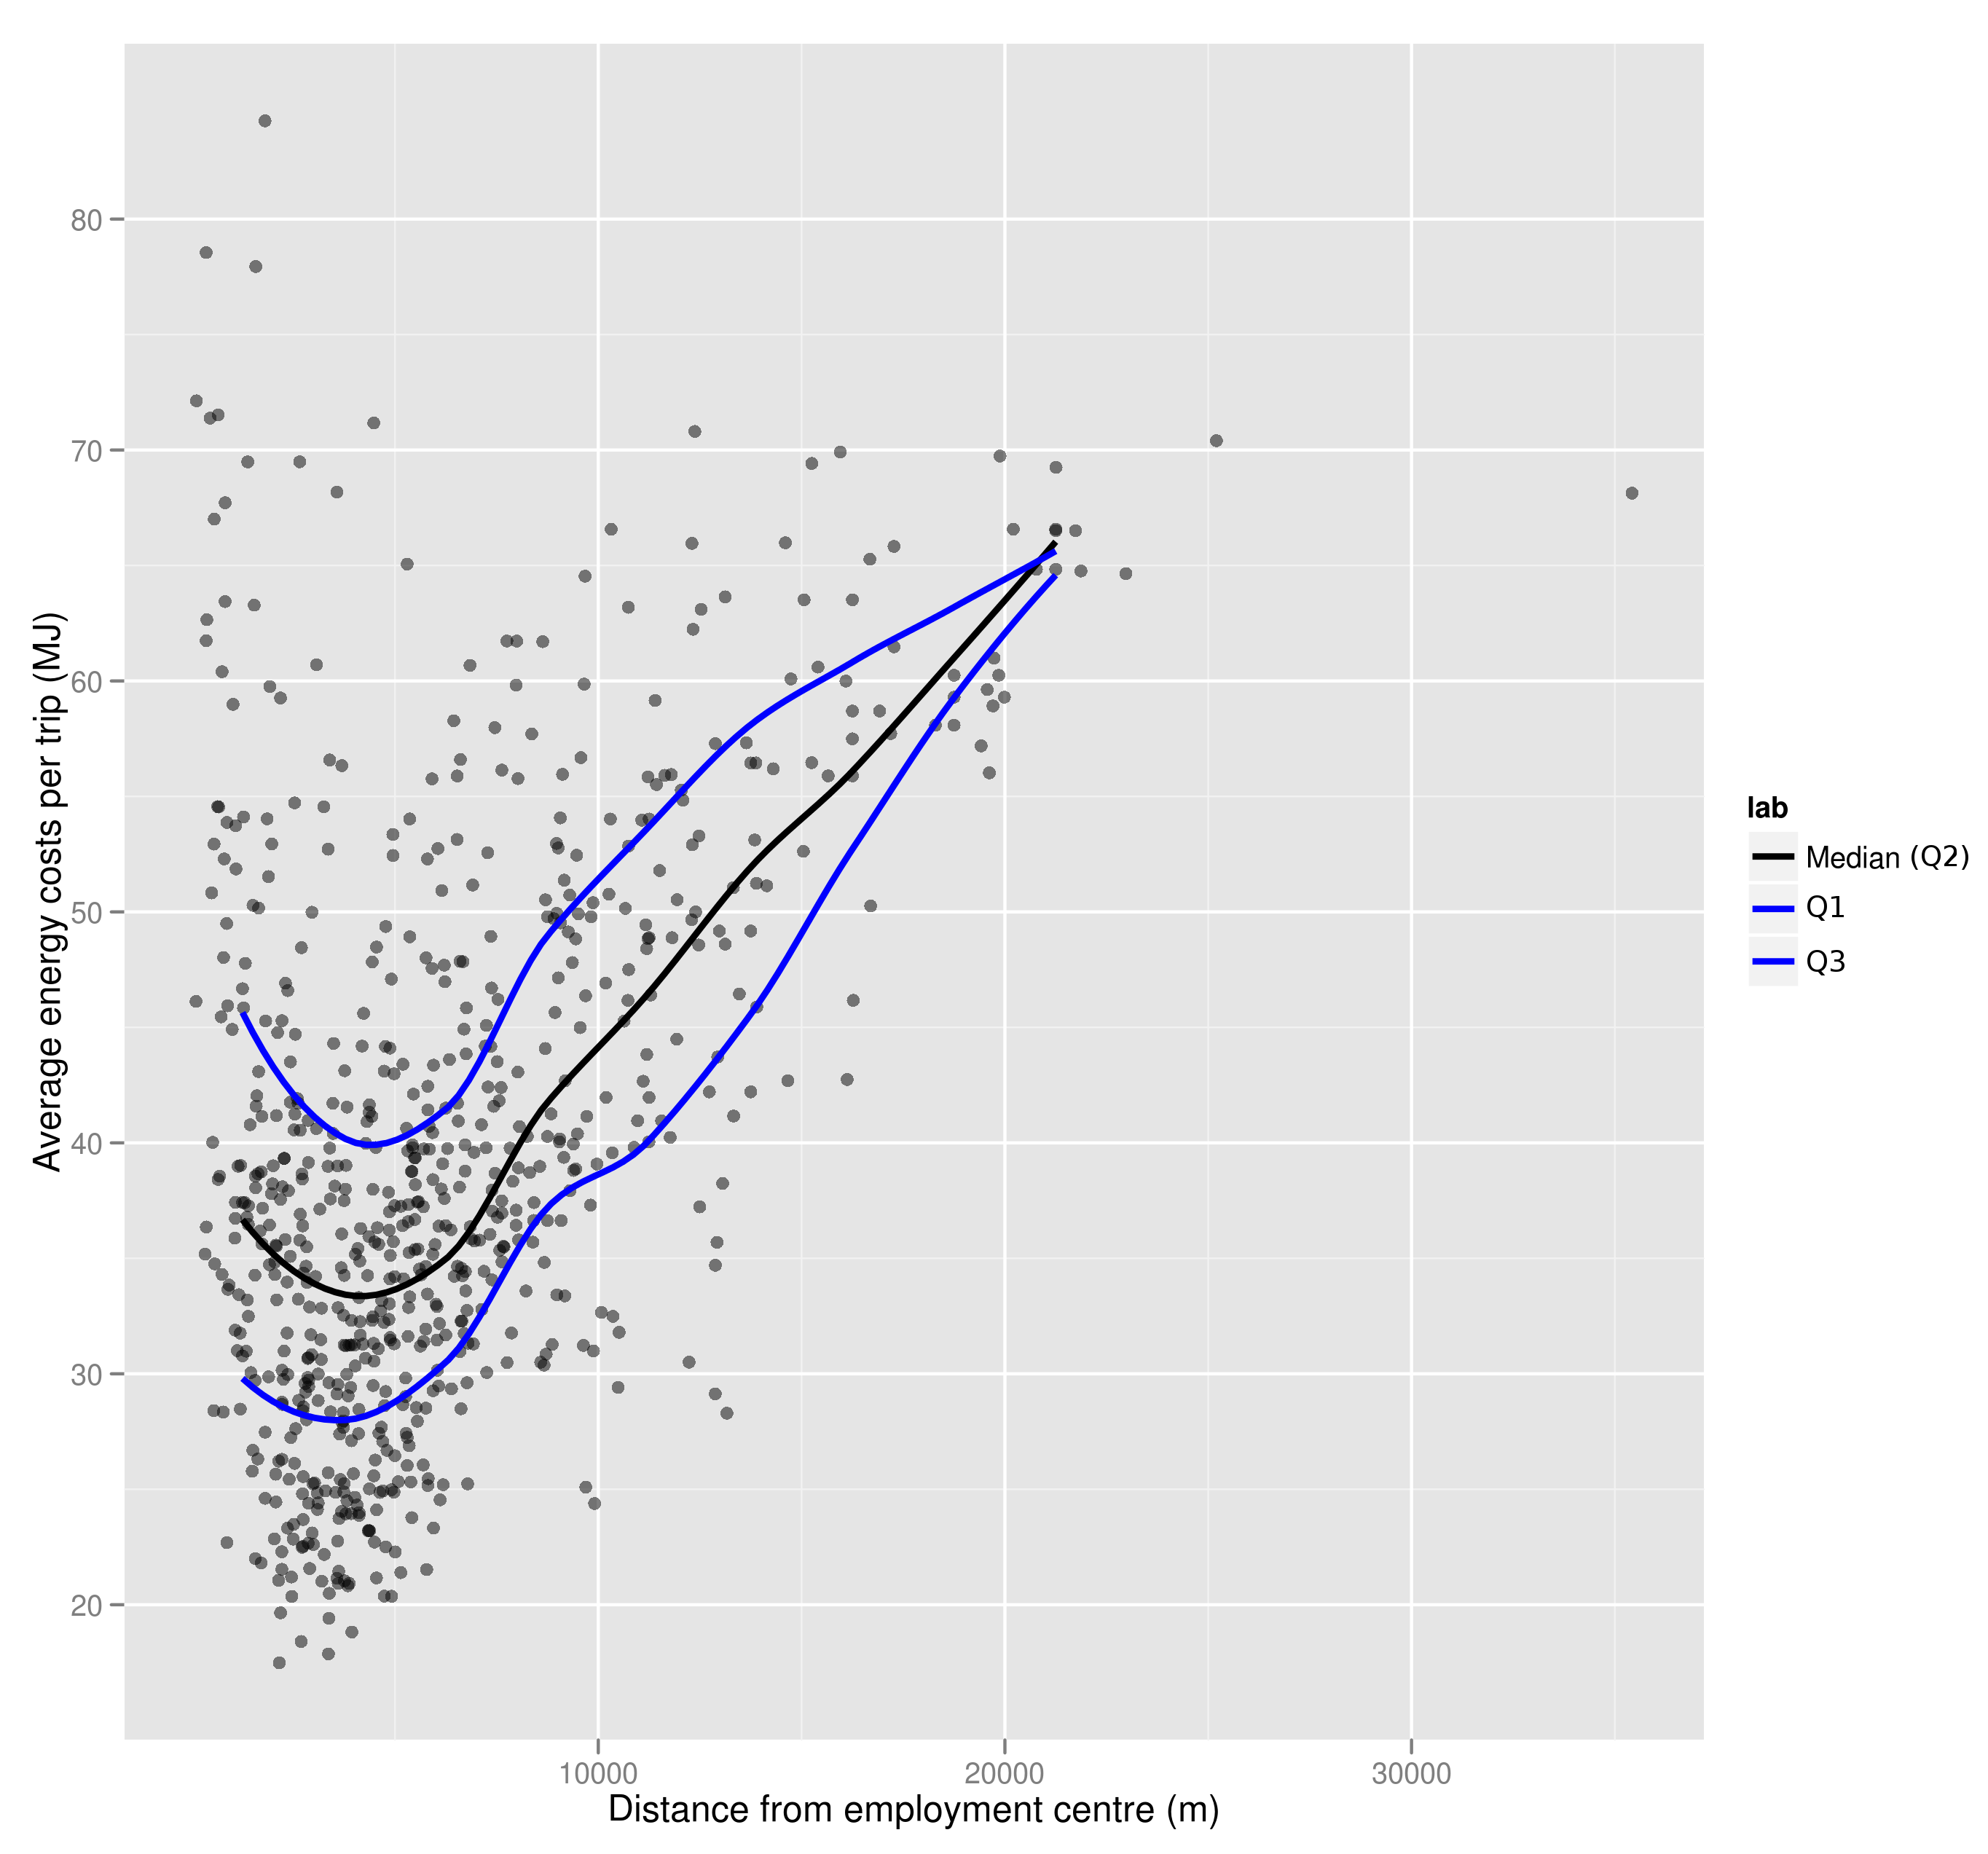
\includegraphics[width=12cm]{Dist-vs-Et2}
 \caption[Scatter plot of distance vs energy costs in Yorkshire and the Humber]
 {The relationship between distance to employment centre and average
energy costs of commute for MSOAs in Yorkshire and the Humber. The blue and
black lines are smoothed moving quantiles (Q1 and Q3 represent the 25$^{th}$ and 75$^{th}$
percentiles respectively), which indicate central tendency and heteroscedasticity.}
 \label{fig:dis-e}
\end{figure}

Spatial microsimulation allows one to `drill down' to the individual
level, target specific groups and model who (in addition to where) is most
likely to benefit from specific interventions. Table \ref{t:msim-res}, for
example, shows simulated differences in commuting patterns between high
and low income citizens in South Yorkshire as a whole.\footnote{The categories
``very poor'' to ``affluent'' used here are defined in \citep{Ballas2005b}.
Statistical bins are defined as proportions of the median income, with
breaks at 50\%, 75\%, 100\% and 125\% of the median \citep[p.~91]{Ballas2005b}.}
Because the individual
microdata are also geocoded, the same analyses could be conducted for
specific zones.
Table \ref{t:msim-res2} illustrates how the results of spatial microsimulation
allow inter- and intra-zone analysis to be combined. Table \ref{t:msim-res2}
indicates that Sheffield028 (an MSOA zone) is more unequal in terms of
income and distance travelled to work than Stocksbridge (a statistical Ward)
(see Fig.~\ref{fig:agent} to see their respective locations).
These results, which can be compared with the regional data presented
in Table \ref{t:msim-res}, or re-calculated for smaller zones, are thus
(to the extent that administrative boundaries allow)
`frame independent' \citep{Horner2002}.

To further explore differences in intra-zone inequality,
commuter work travel distances were plotted as Lorenz curves
(Fig.~\ref{fig:cat-vars}b).
These provide further insight into commuter patterns in each of the zones
described in Table \ref{t:msim-res2}, and illustrate that a small proportion of
the population living in Crookes accounts for a large part of the average trip
distance. Stocksbridge, by contrast, has a more even distribution of commuter
patterns.

Regarding the categorical target variables described in Table \ref{t:indata},
the results imply that wealthy commuters in South Yorkshire drive larger cars,
use the internet more frequently, and may be less likely to want to move
than those with low incomes (Fig.~\ref{fig:cat-vars}a).

\begin{table}[h*]
\caption[Contingency table of variables related to commuting]
{Contingency table of average values for continuous variables related to commuting,
cross-tabulated by income bands, based on the spatial microsimulation
model for South Yorkshire (n = 531,282).}
\begin{center}
\begin{tabular}{lrrrrrr}
\hline
Income group & \multicolumn{1}{l}{Proportion} & \multicolumn{1}{l}{Age} &
\multicolumn{1}{l}{Dis (km)} & \multicolumn{1}{l}{N.cars} &
\multicolumn{1}{l}{Income (\pounds/yr)} & \multicolumn{1}{l}{N.child} \\
\midrule
v.poor & 10\% & 38 & 5.8 & 1.2 & 5519 & 0.9 \\ 
poor & 18\% & 39 & 8.1 & 1.2 & 10158 & 1.0 \\ 
below.av & 22\% & 39 & 8.3 & 1.4 & 13974 & 0.8 \\ 
above.av & 18\% & 39 & 8.9 & 1.6 & 17902 & 0.6 \\ 
affluent & 32\% & 40 & 16.5 & 1.9 & 29448 & 0.5 \\ 
\end{tabular}\end{center}
\label{t:msim-res}
\end{table}

\begin{table}[h*]
\caption[Commuting characteristics cross-tabulated by income bands]
{Contingency table of average values for continuous variables related to commuting,
cross-tabulated by income bands, based on the spatial microsimulation
model for the Ward of Stocksbridge (n = 6,338) and MSOA Sheffield028, which
corresponds to Crookes (n = 2,470).}
\begin{center}
\begin{tabular}{lrrrrrr}
\toprule
Income group & \multicolumn{1}{l}{Proportion} & \multicolumn{1}{l}{Age} &
\multicolumn{1}{l}{Dis (km)} & \multicolumn{1}{l}{N.cars} &
\multicolumn{1}{l}{Income(\pounds/yr)} & \multicolumn{1}{l}{N.child} \\ \midrule
\multicolumn{7}{c}{Stocksbridge (13 km from centre)} \\ \midrule
v.poor & 10\% & 39 & 9.5 & 1.2 & 5886 & 1.0 \\ 
poor & 21\% & 38 & 12.3 & 1.0 & 10571 & 0.9 \\ 
below.av & 19\% & 39 & 12.3 & 1.5 & 14560 & 0.7 \\ 
above.av & 20\% & 39 & 12.9 & 1.8 & 18513 & 0.5 \\ 
affluent & 30\% & 40 & 17.1 & 2.0 & 29198 & 0.5 \\ \midrule
\multicolumn{7}{c}{Crookes (2 km from centre)} \\ \midrule
v.poor &  10\% & 32 & 4.0 & 1.1 & 5208 & 0.8 \\ 
poor & 16\% & 33 & 5.7 & 0.9 & 9972 & 0.9 \\ 
below.av & 23\% & 31 & 7.4 & 1.1 & 14145 & 0.5 \\ 
above.av & 14\% & 34 & 8.7 & 1.5 & 17914 & 0.5 \\ 
affluent & 37\% & 36 & 25.0 & 1.8 & 29932 & 0.4 \\
\bottomrule
\end{tabular}             \end{center}
\label{t:msim-res2}
\end{table}

\begin{figure}[h*]
 \centering
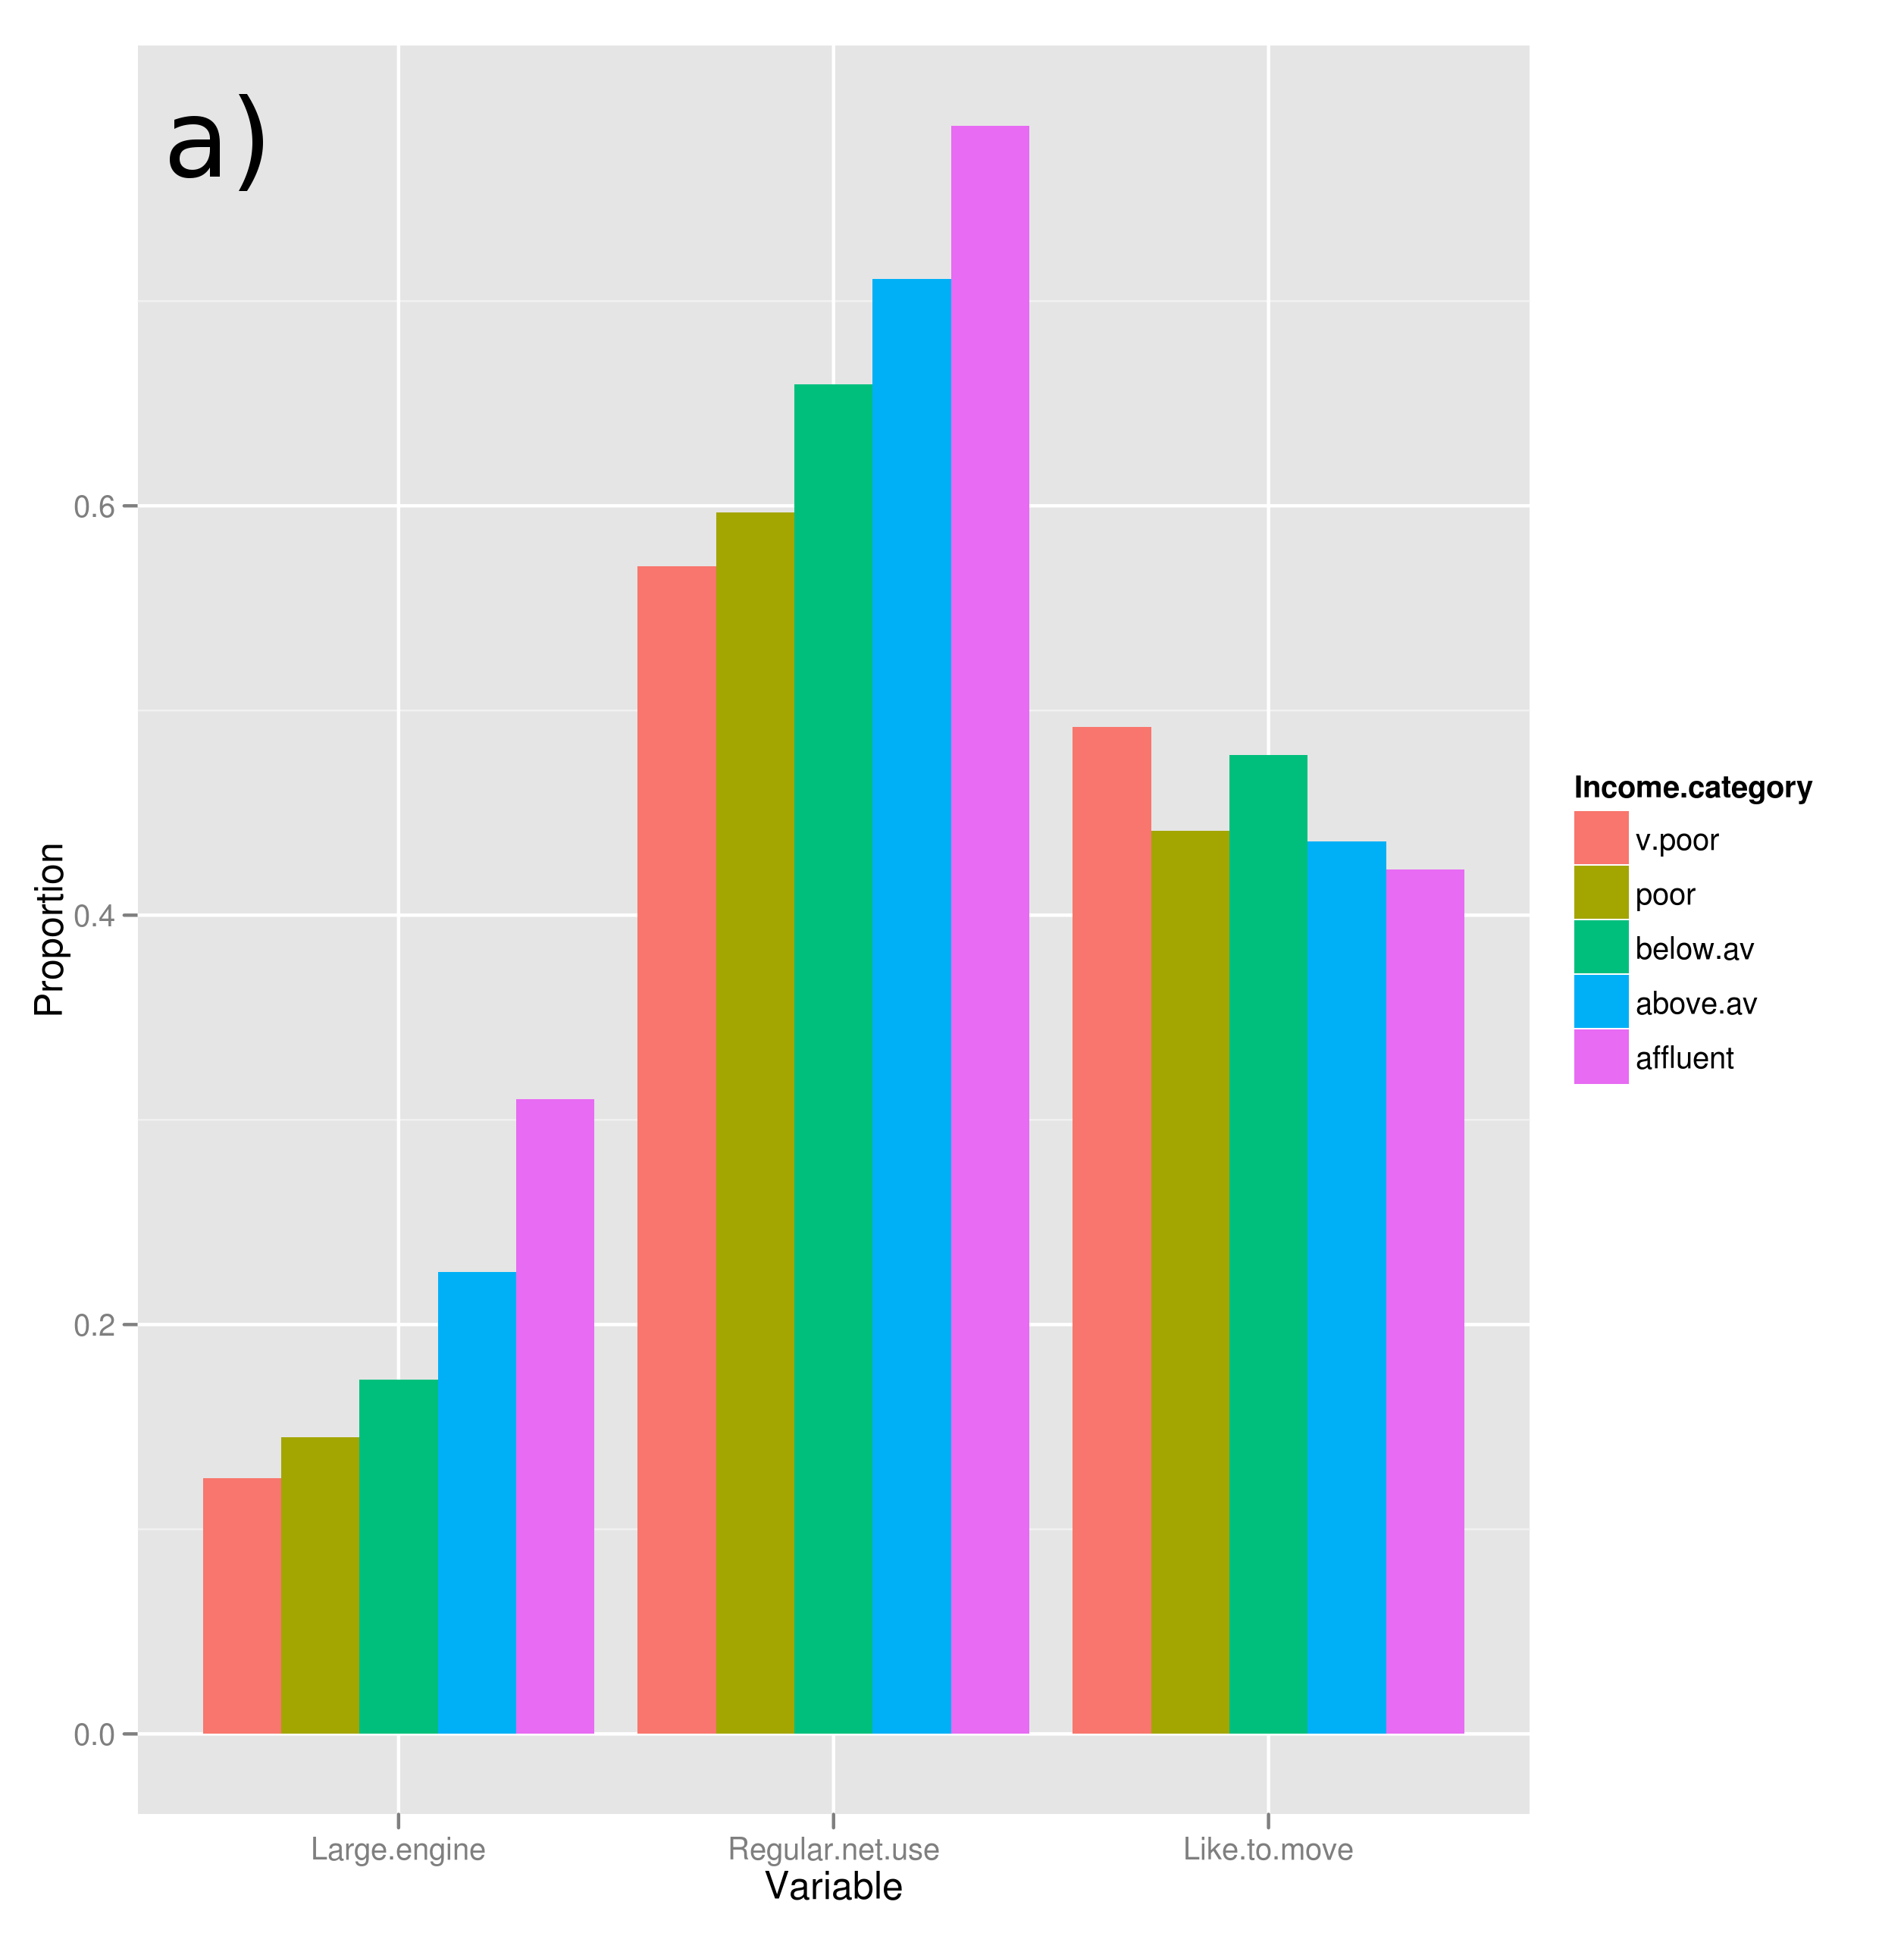
\includegraphics[width=8.2cm]{cat-vars}
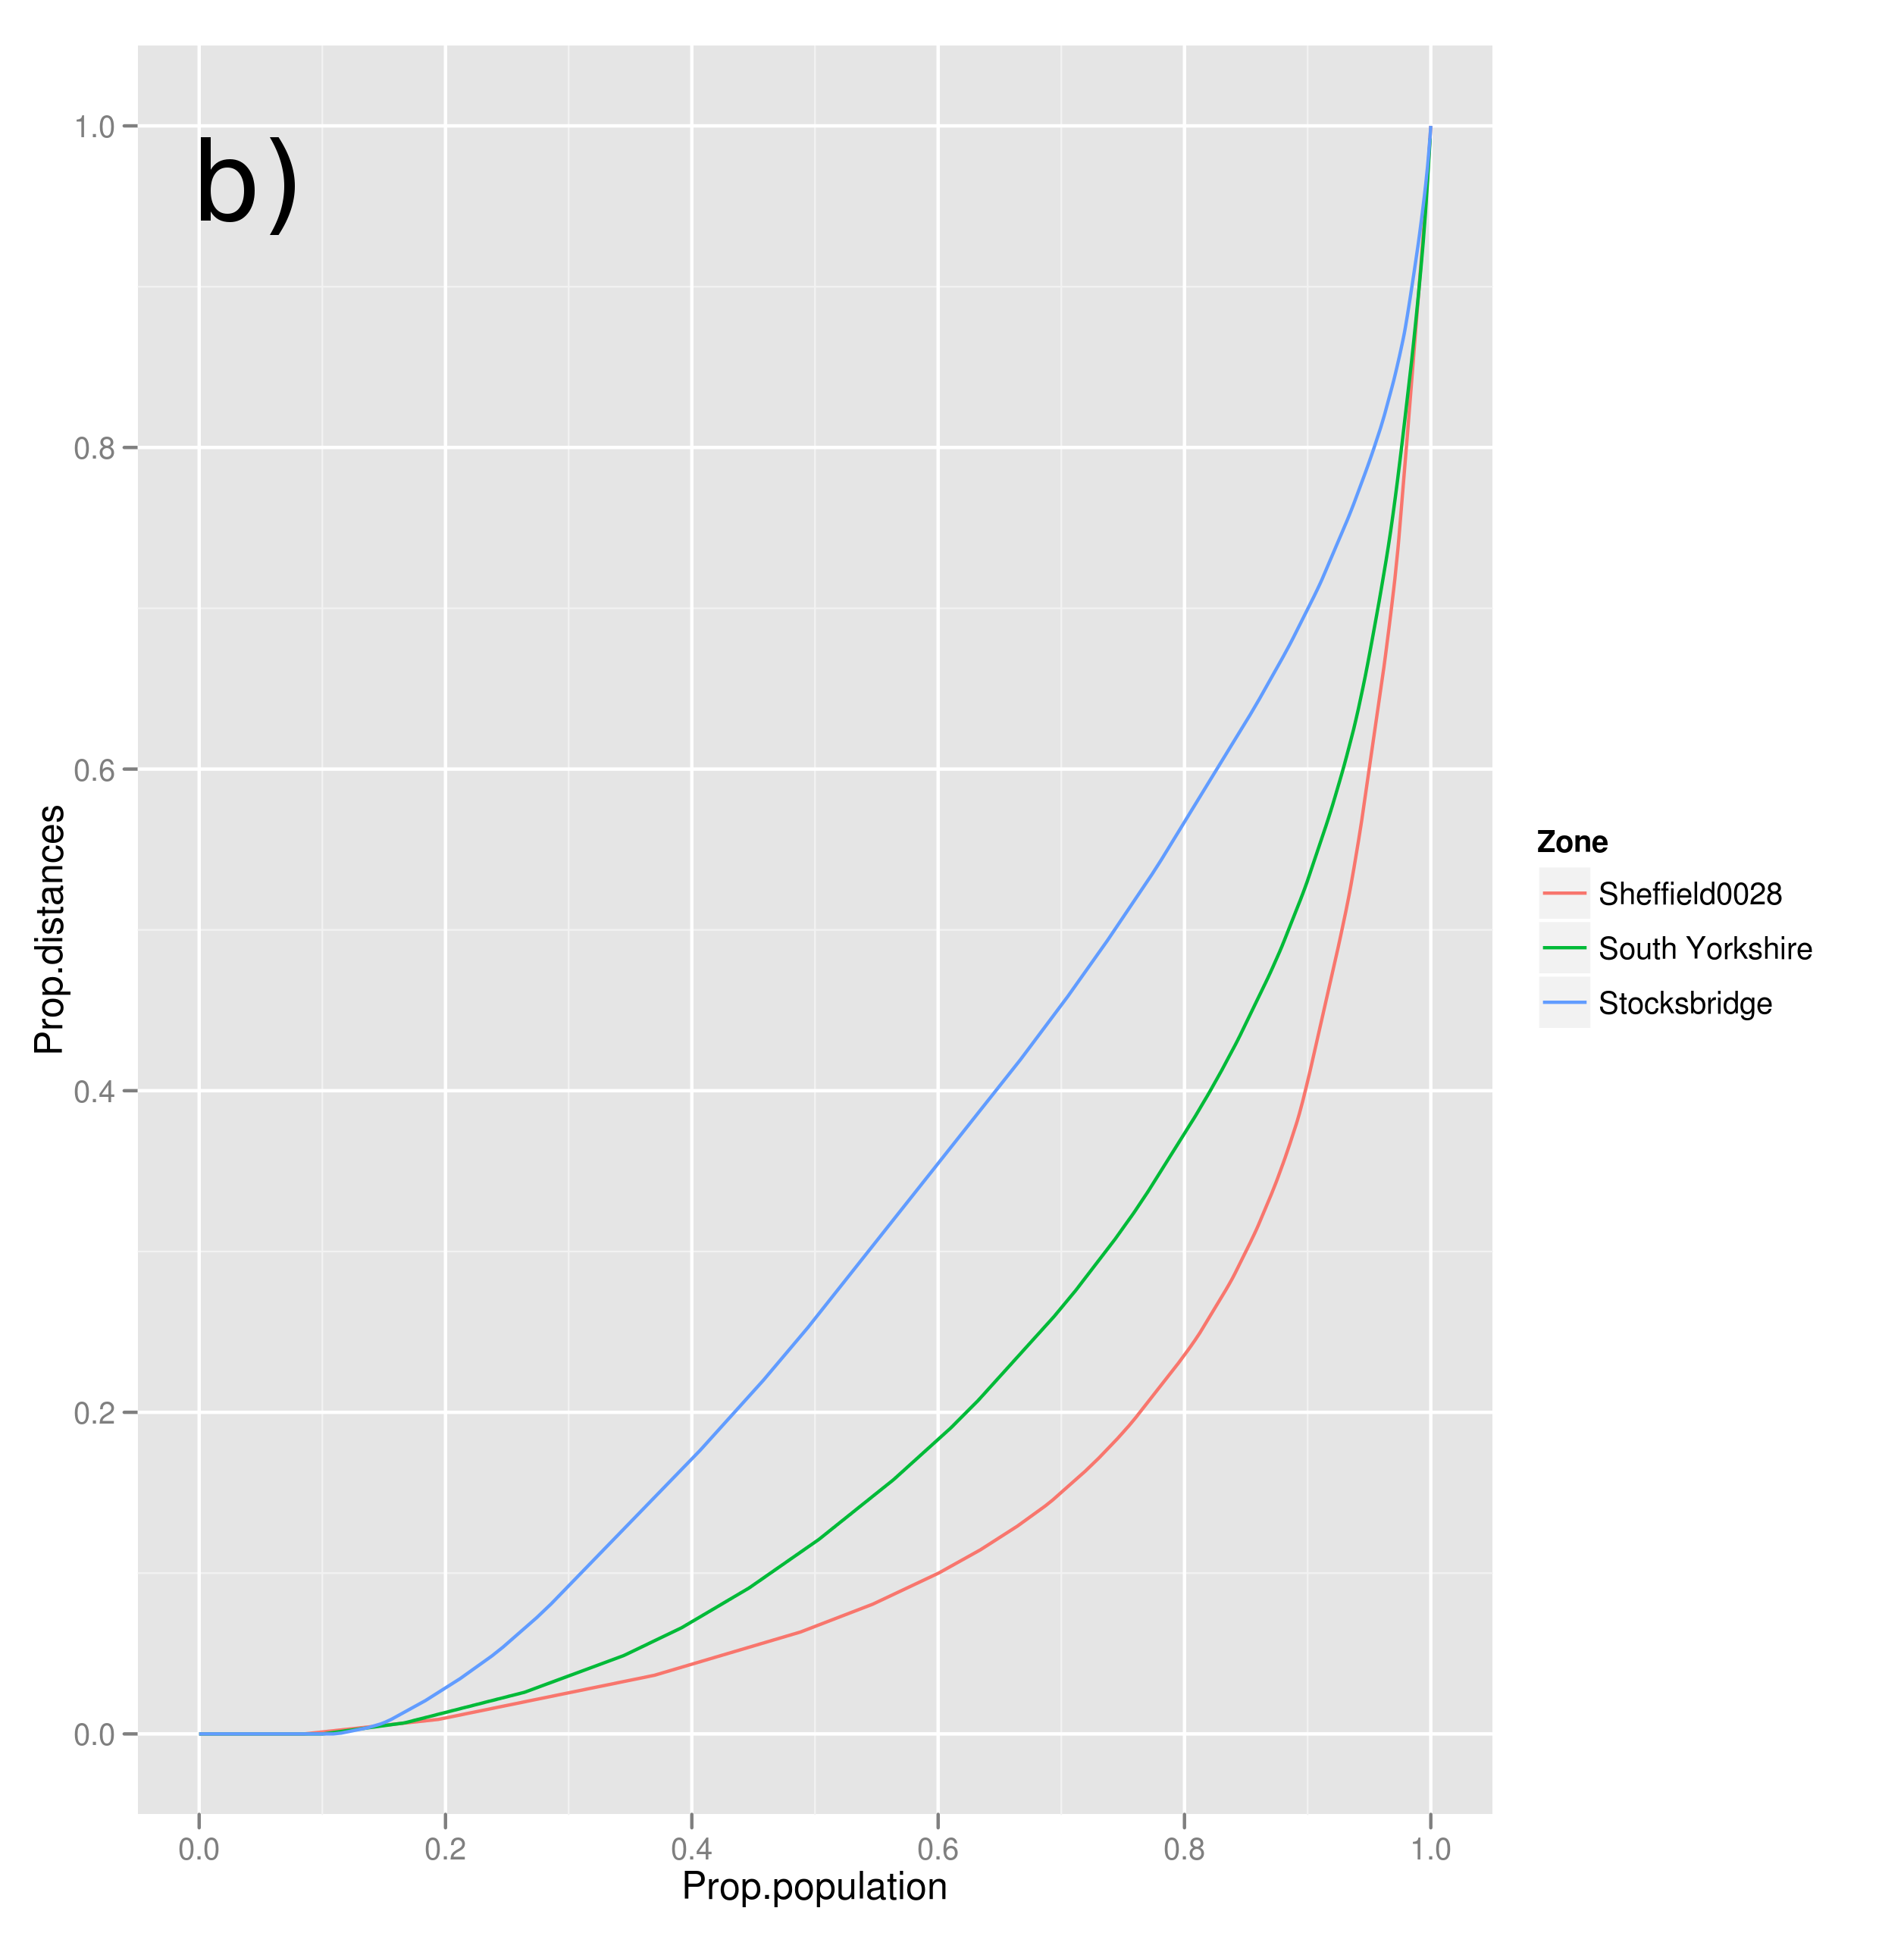
\includegraphics[width=8.2cm]{Lorenz3}
 \caption[a) Income and household traits; b) Lorenz curves of commute distances]
 {\textbf{a)} Variability of vehicles (proportion of primary cars in household
whose engine size is 2.0 litres or more), internet use (proportion of
commuters who use the internet daily or weekly) and desire to move home
depending on equivalised income. These categorical target variables are
described in Table \ref{t:indata}. \textbf{b)} Lorenz curves illustrating the
individual level variability in
commuter distances for 3 zones. The Gini indices associated with these curves
are 0.278, 0.294 and 0.305 for Stocksbridge, South Yorkshire and Sheffield028
respectively.}
 \label{fig:cat-vars}
\end{figure}

\section{Discussion}
\label{discuss-jtrg}
This chapter has demonstrated how spatial microsimulation can be
used to model commuter patterns in concrete case study.
Whole individuals from a detailed national survey were
allocated to geographic zones at various levels; this provided further insight
into intra-zone variability of commuting than is available from the use of
aggregated census data alone. In addition, the careful selection of target
variables not included in the census provided insight into the relationships
between commuting behaviour and a variety of `target variables' such as income,
internet use, desire to move home, type of car and number of children.

From the perspective of data-constrained policy makers, these results are attractive:
they provide a level of detail that is inaccessible for analyses
based on geographically aggregated census data alone. The ability
to explore the commuter behaviour of subsets of individuals based on age,
distance travelled and class (constraint variables) or other variables
including size of car or income (target variables) will be useful in
various applications:
being able to simulate the \emph{characteristics} of commuters who are most
likely to benefit from certain interventions and identifying \emph{where} these
people live and work clearly has huge potential for transport planning and policy.
To illustrate the point, the
distribution of low-income households reliant on buses can be simulated and mapped
at the county level to help inform the location of new bus routes (Fig.
\ref{fig:busmap}). For example, if this type of analysis had been properly
conducted and validated during the planning stages of the recently implemented
rapid bus routes in Albuquerque mentioned in \citet{Tribby2012},
the system could have been
designed such that low income residents benefited from faster access to the city
centre. In fact, relatively wealthy households (who probably have more transport
options already) benefited most from the scheme \citep{Tribby2012}. This
illustrates the importance of considering not only aggregate level impacts, but
also taking into account the local and micro level distributional effects of
intervention.

\begin{figure}[h*]
 \centering
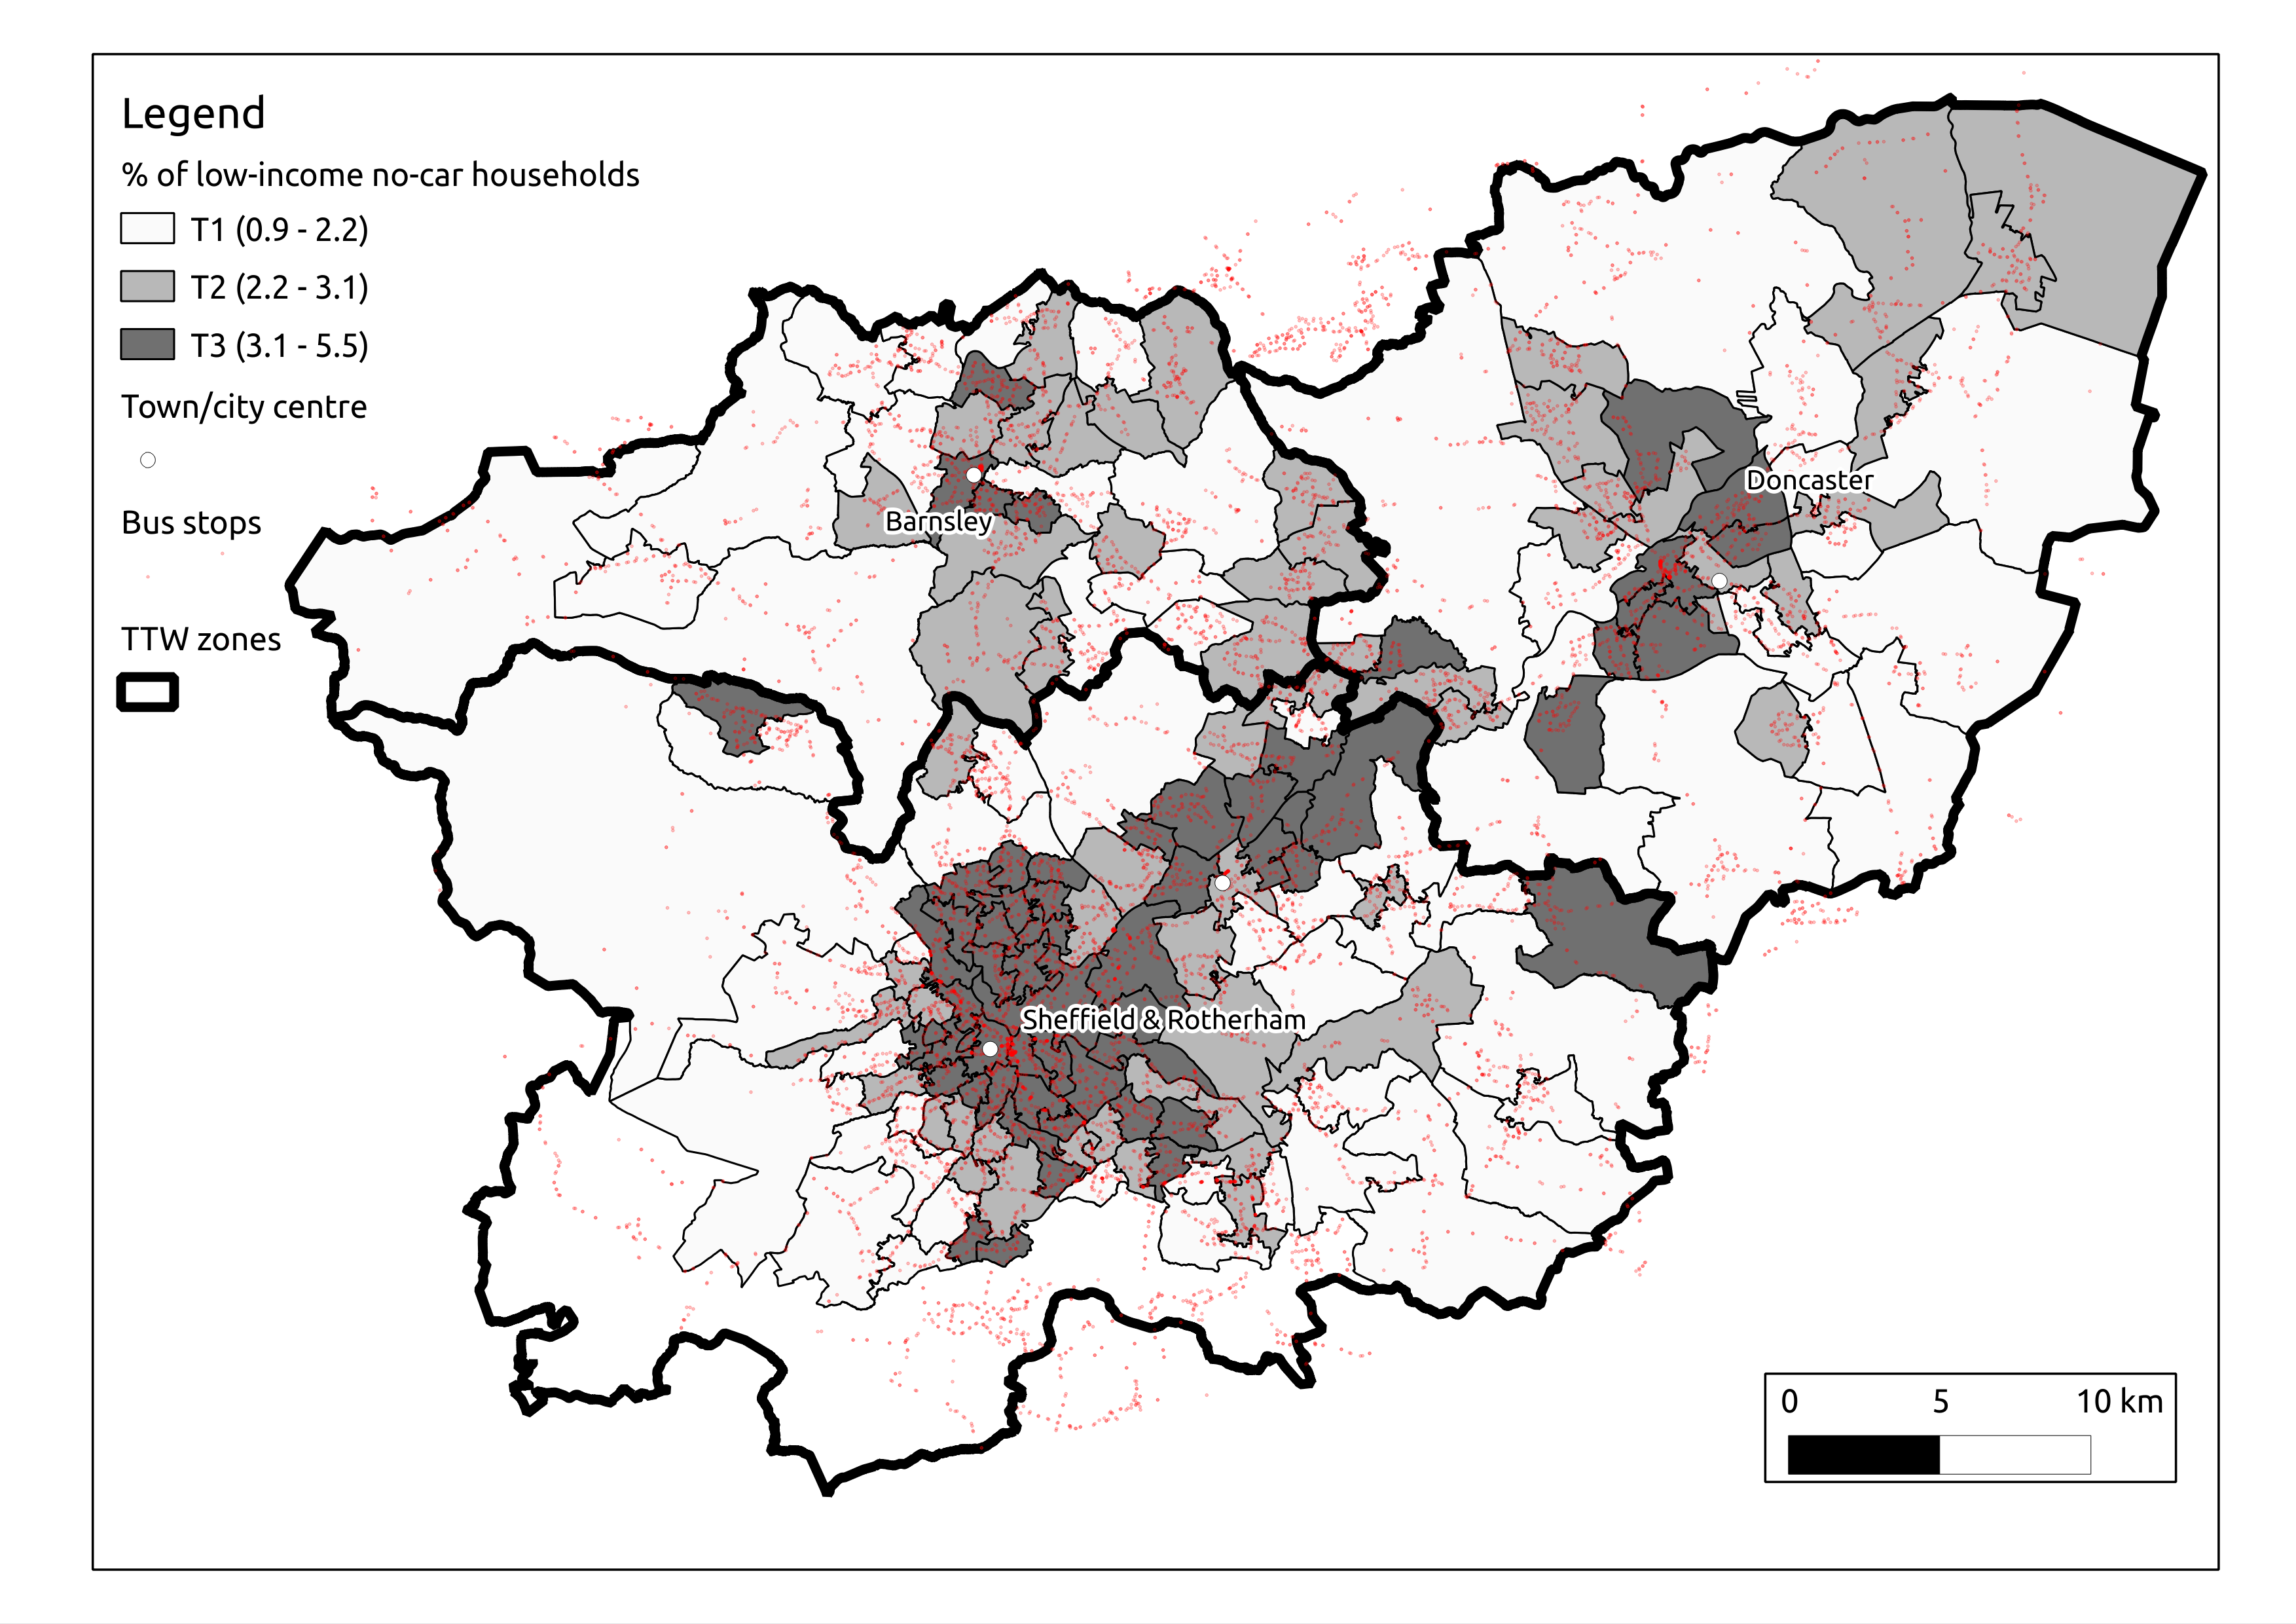
\includegraphics[width=13.5cm]{busmap}
 \caption[Low-income car-free families and bus-stops in South Yorkshire]
 {Proportion of population which earns less than 50\% of South
Yorkshire's median income \emph{and} lives in a car free household within the 173 MSOA
boundaries of the metropolitan county, according to the spatial
microsimulation model. Translucent red dots represent bus
stops (data from {\color{blue}\href{http://data.gov.uk/dataset/nptdr}{data.gov.uk/dataset/nptdr}}).}
 \label{fig:busmap}
\end{figure}

The spatial microsimulation approach to modelling commuter
patterns outlined in this section provides a foundation for investigating such
effects.  In addition, it has been shown that spatial microsimulation methods
can enrich transport models with policy relevant socio-economic variables at
individual and small-area levels.
% In broader terms,
% the  promotes a closer collaboration between the fields of
% transport modelling, spatial microsimulation and spatial microsimulation.

Despite these possibilities, it is important to remember that the results are
\emph{simulated}. Consequently, 
linking variables --- these
are constrained by known census aggregates and are therefore trustworthy ---
must be distinguished from target variables, which are more tentative
estimates based on correlations between target and linking
variables at the national level. Target variable
estimates rely on an often unstated assumption: that the relationships
between variables at the national level (e.g.~between distance travelled to
work and income) tend to remain at local levels. This assumption cannot be
expected to hold everywhere, so results arising from target variables are
expected to underplay the true level of spatial variability. Where possible,
target variable results should be corroborated against independent datasets
(\citealp{Edwards2009}).

Many transport interventions have wide-ranging impacts on commuters.
These depend on geographical \emph{and} individual level factors,
and the importance of the latter especially is often overlooked in transport policy
 (e.g.~\citealp{Tribby2012}).
The micro level methods presented in this chapter therefore have great potential,
to enable researchers and transport planners to better model and predict the
impacts arising from various interventions.
With the current focus on energy and sustainability in transport
\citep{Chapman2007}, there is a risk that distributional impacts continue
to receive little or no attention. Spatial microsimulation
has the potential to address this issue, by helping
decision makers to design sustainable transport measures
that are both effective and fair.
